% =====================================================================
%  AB02 - complete documentation (single PDF)
%  Build:  pdflatex AB02_Drone_Documentation.tex   (run it twice for the contents)
%  Figures are read from ../figures (Python scripts), ../mathematical_models/figures
%  (flow diagrams) and ../../toy_model/figures (MATLAB toy model); the code
%  listings are read directly from the repository files.
% =====================================================================
\documentclass[11pt,a4paper]{article}
\usepackage[a4paper, margin=2.2cm, headheight=14pt]{geometry}
% =====================================================================
%  Shared preamble of the AB02 documents (complete documentation and
%  mathematical models). \input from both main files.
% =====================================================================
\IfFileExists{lmodern.sty}{\usepackage[T1]{fontenc}\usepackage{lmodern}}{}
\usepackage{microtype}
\usepackage{amsmath,amssymb,amsthm,bm,mathtools}
\usepackage{graphicx}
\usepackage{booktabs,array,tabularx,longtable,multirow}
\usepackage{xcolor}
\usepackage[most]{tcolorbox}
\usepackage{enumitem}
\usepackage{fancyhdr}
\usepackage{titlesec}
\usepackage{caption}
\usepackage{float}
\usepackage{listings}
\usepackage{needspace}
\usepackage{tikz}
\usetikzlibrary{arrows.meta, positioning, calc, fit, backgrounds}
\usepackage[hidelinks]{hyperref}
\usepackage[nameinlink]{cleveref}

% ---------------------------------------------------------------- colours
\definecolor{cHead}{HTML}{0D3B66}
\definecolor{cText}{HTML}{263238}
\definecolor{cPlant}{HTML}{37474F}
\definecolor{cEnv}{HTML}{A0620F}
\definecolor{cCtrl}{HTML}{AD1457}
\definecolor{cAdapt}{HTML}{4527A0}
\definecolor{cX3}{HTML}{1565C0}
\definecolor{cOk}{HTML}{2E7D32}
\definecolor{cWarn}{HTML}{B23A48}
\definecolor{cCodeBg}{HTML}{F4F4F4}
\definecolor{cKey}{HTML}{0000FF}
\definecolor{cCom}{HTML}{228B22}
\definecolor{cStr}{HTML}{A020F0}
\hypersetup{colorlinks=true, linkcolor=cHead, urlcolor=cX3, citecolor=cHead}

% ---------------------------------------------------------------- headings
\titleformat{\section}{\Large\sffamily\bfseries\color{cHead}}{\thesection}{0.8em}{}[{\color{cHead}\titlerule[0.8pt]}]
\titleformat{\subsection}{\large\sffamily\bfseries\color{cHead}}{\thesubsection}{0.7em}{}
\titleformat{\subsubsection}{\normalsize\sffamily\bfseries\color{cText}}{\thesubsubsection}{0.6em}{}
\titlespacing*{\section}{0pt}{2.2ex plus 1ex}{1.4ex}
\titlespacing*{\subsection}{0pt}{2.0ex plus 1ex}{1.0ex}

\setlist{itemsep=2pt, topsep=4pt}
\setlength{\parindent}{0pt}
\setlength{\parskip}{5pt}
\captionsetup{font=small, labelfont={bf,sf}}
\renewcommand{\arraystretch}{1.15}

% ---------------------------------------------------------------- notation
\newcommand{\vq}{\bm{q}}  \newcommand{\qv}{\bm{q}_v} \newcommand{\vw}{\bm{\omega}}
\newcommand{\vu}{\bm{u}}  \newcommand{\vd}{\bm{d}}   \newcommand{\vs}{\bm{s}}
\newcommand{\vtau}{\bm{\tau}} \newcommand{\veps}{\bm{\varepsilon}} \newcommand{\vF}{\bm{F}}
\newcommand{\vp}{\bm{p}}  \newcommand{\vv}{\bm{v}}  \newcommand{\ve}{\bm{e}}
\newcommand{\vx}{\bm{x}}  \newcommand{\vr}{\bm{r}}
\newcommand{\that}{\hat{\theta}} \newcommand{\ttil}{\tilde{\theta}}
\newcommand{\skw}[1]{#1^{\times}}
\newcommand{\R}{\mathbb{R}}
\newcommand{\sat}{\operatorname{sat}}
\newcommand{\sgn}{\operatorname{sgn}}
\newcommand{\diag}{\operatorname{diag}}
\newcommand{\umax}{u_{\max}}
\newcommand{\cbreakus}{\textunderscore\allowbreak}
\newcommand{\code}[1]{{\ttfamily\small\let\_\cbreakus #1}}

% ---------------------------------------------------------------- boxes
\tcbset{base/.style={enhanced, breakable, boxrule=0.7pt, arc=2.5pt, left=7pt, right=7pt,
  top=5pt, bottom=5pt, fonttitle=\sffamily\bfseries\small, before skip=8pt, after skip=8pt,
  before upper={\setlength{\parskip}{4pt}}}}
\newtcolorbox{eqbox}[2]{base, colback=#1!4, colframe=#1, colbacktitle=#1, coltitle=white, title={#2}}
\newtcolorbox{toybox}[1][]{base, colback=cEnv!5, colframe=cEnv!70, colbacktitle=cEnv!14,
  coltitle=cEnv!80!black, title={Toy example\ifx&#1&\else\ --- #1\fi}}
\newtcolorbox{idea}[1][]{base, colback=cX3!4, colframe=cX3!55, colbacktitle=cX3!12,
  coltitle=cX3!80!black, title={\ifx&#1&The idea in plain words\else #1\fi}}
\newtcolorbox{projbox}[1][]{base, colback=cOk!5, colframe=cOk!70, colbacktitle=cOk!14,
  coltitle=cOk!70!black, title={In our project\ifx&#1&\else\ --- #1\fi}}
\newtcolorbox{warn}[1][]{base, colback=cWarn!5, colframe=cWarn!80, colbacktitle=cWarn!15,
  coltitle=cWarn!80!black, title={\ifx&#1&Be careful\else #1\fi}}
\newtcolorbox{codebox}{base, colback=cPlant!4, colframe=cPlant!45, boxrule=0.5pt,
  fontupper=\small, left=6pt, top=3pt, bottom=3pt}

% symbol table:  \begin{dimtable} sym & meaning & dimension & unit \\ \end{dimtable}
\newenvironment{dimtable}{%
  \par\smallskip\small
  \tabularx{\linewidth}{@{}>{$}l<{$} X >{$}l<{$} l@{}}
  \toprule
  \textrm{\textbf{Symbol}} & \textbf{Meaning} & \textrm{\textbf{Dimension}} & \textbf{Unit}\\
  \midrule}{%
  \bottomrule\endtabularx\par\smallskip}

% ---------------------------------------------------------------- code listings
\lstdefinestyle{common}{basicstyle=\ttfamily\footnotesize, backgroundcolor=\color{cCodeBg},
  frame=single, rulecolor=\color{black!20}, framesep=4pt, xleftmargin=6pt, xrightmargin=2pt,
  keywordstyle=\color{cKey}, commentstyle=\color{cCom}, stringstyle=\color{cStr},
  showstringspaces=false, breaklines=true, columns=fullflexible, keepspaces=true,
  numberstyle=\tiny\color{black!50}, aboveskip=6pt, belowskip=6pt, upquote=true}
\lstdefinestyle{py}{style=common, language=Python, numbers=left, numbersep=6pt}
\lstdefinestyle{mat}{style=common, language=Matlab}
\lstdefinestyle{sh}{style=common, language=bash}

% ---------------------------------------------------------------- toy-model figure
% \toyfig{file.png}{width}{caption}{label}: figure produced by toy_model/run_all.m (MATLAB).
\newcommand{\toyfig}[4]{%
  \begin{figure}[H]\centering
  \IfFileExists{../../toy_model/figures/#1}{\includegraphics[width=#2]{../../toy_model/figures/#1}}{%
    \fbox{\parbox{0.8\linewidth}{\centering\vspace{1.2cm}\sffamily\small
      \texttt{toy\_model/figures/\detokenize{#1}}\\ is created by \texttt{toy\_model/run\_all.m} (MATLAB).\vspace{1.2cm}}}}
  \caption{#3 \emph{(MATLAB toy model, \texttt{toy\_model/figures/\detokenize{#1}}.)}}\label{#4}
  \end{figure}}
% \resfig{file.png}{width}{caption}{label}: figure produced by the Python scripts (docs/figures).
\newcommand{\resfig}[4]{%
  \begin{figure}[H]\centering\includegraphics[width=#2]{../figures/#1}
  \caption{#3}\label{#4}\end{figure}}

% ---------------------------------------------------------------- code read straight from the repository
% \pyfile{first line}{last line}{file}{title}
\newcommand{\pyfile}[4]{\lstinputlisting[style=py, firstline=#1, lastline=#2, firstnumber=#1,
  title={\small\sffamily #4}]{#3}}
\newcommand{\matfile}[4]{\lstinputlisting[style=mat, numbers=left, numbersep=6pt, firstline=#1, lastline=#2,
  firstnumber=#1, title={\small\sffamily #4}]{#3}}
\newcommand{\repro}{../../paper_reproduction.py}
\newcommand{\xmodel}{../../x3_sim/x3_model.py}
\newcommand{\xctrl}{../../x3_sim/controllers.py}
\newcommand{\xrun}{../../x3_sim/run_x3_experiments.py}
\newcommand{\gznode}{../../gazebo.py}
\newcommand{\toylib}{../../toy_model/lib}
\newcommand{\toydir}{../../toy_model}

\graphicspath{{../figures/}{../mathematical_models/figures/}}

\pagestyle{fancy}
\fancyhf{}
\fancyhead[L]{\small\sffamily\color{cText!70}AB02 \,|\, complete documentation}
\fancyhead[R]{\small\sffamily\color{cText!70}\nouppercase{\leftmark}}
\fancyfoot[C]{\small\sffamily\thepage}
\renewcommand{\headrulewidth}{0.4pt}

\begin{document}

\begin{titlepage}
  \centering
  \vspace*{1.0cm}
  {\includegraphics[width=0.36\linewidth]{../../amrita.png}\\[18pt]}
  {\Huge\sffamily\bfseries\color{cHead} A Simple Structure Constrained\\[4pt] Attitude Control for Rigid Bodies\\[10pt]}
  {\Large\sffamily\color{cText} Implementation, reproduction and quadcopter integration\\ of a PD-type prescribed-performance controller\\[22pt]}
  {\large\sffamily Introduction to Drones -- 22AIE448\\[20pt]}
  {\large\sffamily\bfseries Group AB02}\\[6pt]
  {\sffamily
  \begin{tabular}{ll}
  Nethra R & CB.SC.U4AIE24147\\
  Dheeraj S & CB.SC.U4AIE24050\\
  Raaman Namputhiri & CB.SC.U4AIE24148\\
  Jyothsna & CB.SC.U4AIE24117
  \end{tabular}}\\[10pt]
  {\sffamily School of Artificial Intelligence, Amrita Vishwa Vidyapeetham, Coimbatore}\\[16pt]
  {\small\sffamily Base paper: M.~Golestani et al., \emph{IEEE Access}, vol.~10, pp.~10202--10209, 2022, DOI 10.1109/ACCESS.2022.3144627}
  \vfill
  \begin{minipage}{0.9\linewidth}\small\color{cText}
  \textbf{What this document is.} One place that explains everything in our project: the base paper's controller, how
  we implemented it, how faithfully we reproduced its simulations (with numbers, not only plots), what we found that the
  paper does not say, and how we carried the controller onto the Gazebo X3 quadcopter, including why our first version
  crashed and how it was fixed. Every number in this document is produced by a script in the repository and can be
  regenerated with the commands of \cref{sec:setup}. The equation-by-equation derivations are in the companion document
  \code{docs/mathematical\_models/Mathematical\_Models.pdf}; every MATLAB toy example is in \code{toy\_model/}.
  \end{minipage}
\end{titlepage}

\tableofcontents
\newpage

% =====================================================================
\section{Read Me First}
\label{sec:readme}
% =====================================================================

\subsection{The project in one paragraph}

The base paper (Golestani et al., IEEE Access 2022) proposes a PD-type attitude controller that keeps \emph{both} the
attitude quaternion and the angular velocity of a rigid body inside time-varying bounds that close in a finite, chosen
time, while the actuators saturate and an unknown disturbance acts. Its selling point is simplicity: an ordinary PD law
plus one barrier-weighted damping term and one scalar adaptive estimate. We (1) implemented every equation of the
paper, (2) reproduced both of its simulation studies quantitatively, (3) wrote an independent MATLAB toy model that
re-derives every block and re-implements the experiments, (4) tested the controller beyond the paper (300-run Monte-Carlo studies, parameter
sensitivity, an alternative barrier form), and (5) integrated it on the Gazebo X3 quadcopter through ROS~2, where we
found and fixed the faults that made our first version crash.

\subsection{Results at a glance}

\begin{center}\small
\begin{tabularx}{\linewidth}{@{}>{\raggedright\arraybackslash}p{4.6cm} X >{\raggedright\arraybackslash}p{2.2cm}@{}}
\toprule
\textbf{Question} & \textbf{Answer (measured)} & \textbf{Where}\\
\midrule
Does our implementation reproduce the paper's Part~1? & Yes. For $T_s=15$\,s and $10$\,s both $\qv$ and $\vw$ stay strictly inside their
envelopes (0\,\% of the time outside; peak $|\varepsilon|=0.871/0.912$ and $0.924/0.942$), and the shorter $T_s$ converges faster
(settling 5.25\,s vs.\ 4.53\,s), as the paper states. & \cref{sec:part1}\\
Does it reproduce Part~2 (constrained vs.\ conventional PD)? & Yes. Same gains, limit, disturbance and initial state: the constrained law
never leaves the envelopes; conventional PD leaves the angular-velocity envelope 27.5\,\% of the time. The constrained
law also uses 36\,\% less torque energy and halves the final rate error. & \cref{sec:part2}\\
Is this a one-off? & No. 300 random initial states in the paper's regime: 97.0\,\% violation-free (95\,\% CI 94.4--98.4) for
the constrained law, 0.0\,\% for PD. & \cref{sec:mc}\\
Can it be checked independently? & The MATLAB toy model re-implements the spacecraft experiments separately
(\code{toy\_model/step6}); \code{docs/make\_crosscheck.py} puts its numbers next to the Python ones (\cref{tab:crosscheck}). & \cref{sec:crosscheck}\\
What did we find that the paper does not say? & Four unstated parameters; Part~2 starts on its own boundary; the barrier is
one-sided; the envelope must be feasible for the actuator; Theorem~1 proves convergence, not envelope invariance. &
\cref{sec:findings}\\
Does it fly a quadcopter? & Yes, after fixing our first node. The paper's law, re-sized for the X3, hovers for 180\,s and flies
a $2\times2$\,m square (4.0\,cm RMS error) on a software-in-the-loop model built from Gazebo's X3 files, with 0\,\% attitude-envelope
violations. The ROS~2 node \code{gazebo.py} runs exactly this controller. & \cref{sec:x3res}\\
Why did the first Gazebo version crash? & Two faults, isolated one by one: a mixer whose signs did not match the X3
(no pitch authority) and an altitude-rate estimate that was never updated. Fixing both gives a stable flight. & \cref{sec:x3fault}\\
\bottomrule
\end{tabularx}
\end{center}

\subsection{The documents and how to read them}

\begin{center}\small
\begin{tabularx}{\linewidth}{@{}l X@{}}
\toprule
\textbf{Document} & \textbf{Content}\\
\midrule
\code{docs/complete\_documentation/} (this PDF) & project, results, code walk-through, X3 integration, claims\\
\code{docs/mathematical\_models/} & every equation: boxed statement, symbol table, derivation, hand-checkable toy example, flow diagrams\\
\code{toy\_model/} & MATLAB scripts (\code{step1}--\code{step8}) that print the toy examples and plot each idea; \code{run\_all.m} runs all of them\\
\code{docs/results/*.md, *.json} & every number of this document, written by the scripts\\
\code{docs/figures/} & every figure of this document, written by the scripts\\
\bottomrule
\end{tabularx}
\end{center}

\textbf{Colour code of the boxes.} \textcolor{cX3}{Blue}: the idea in plain words. \textcolor{cEnv}{Orange}: a toy
example with numbers. \textcolor{cOk}{Green}: what it means in our project. \textcolor{cWarn}{Red}: something to be
careful about.

\textbf{Naming of the controllers.} Throughout, \emph{constrained (paper Eq.~13)} is the paper's law exactly as printed;
\emph{constrained (symmetric barrier)} is our variant with $(1-\varepsilon^2)^{-2}$ in place of $(1-\varepsilon)^{-2}$
(\cref{sec:barrierform}); \emph{conventional PD} is the same law with $\vu_{cons}=0$, i.e.\ the paper's Part~2 baseline.

% =====================================================================
\section{Project Set-up and How to Reproduce Everything}
\label{sec:setup}
% =====================================================================

\subsection{Repository map}

\begin{center}\small
\begin{tabularx}{\linewidth}{@{}>{\raggedright\arraybackslash}p{5.4cm} X@{}}
\toprule
\textbf{Path} & \textbf{What it is}\\
\midrule
\code{base paper.pdf} & the base paper\\
\code{paper\_reproduction.py} & reproduction of the paper's Section IV (Part 1, Part 2), sensitivity, Monte-Carlo; writes \code{docs/figures/fig*.png}, \code{docs/results/metrics.*}\\
\code{x3\_sim/x3\_model.py} & software-in-the-loop surrogate of the Gazebo X3 (all constants from the Gazebo model files)\\
\code{x3\_sim/controllers.py} & \code{OriginalGazeboController} (exact port of our first node) and \code{FixedController} (the corrected paper controller)\\
\code{x3\_sim/run\_x3\_experiments.py} & experiments E0--E5 on the X3; writes \code{docs/figures/x3\_*.png}, \code{docs/results/x3\_metrics.*}\\
\code{gazebo.py} & ROS~2 node (v2) that flies the Gazebo X3 with \code{FixedController}\\
\code{plot\_gazebo\_log.py} & turns a log of \code{gazebo.py} into figures and metrics\\
\code{tests/test\_gazebo\_node\_offline.py} & runs the real \code{gazebo.py} without ROS against the surrogate\\
\code{toy\_model/} & MATLAB toy model, steps 1--8, \code{run\_all.m}, \code{lib/}\\
\code{Drones\_Mujoco\_*.ipynb}, \code{One\_drone\_alligning.ipynb} & MuJoCo 3-D attitude and flight demos\\
\code{index.html}, \code{app.js}, \code{simulation.js}, \code{style.css} & interactive browser simulator (illustration)\\
\code{legacy/} & first versions kept for the record (\code{gazebo\_v1.py}, early drafts); not used as evidence\\
\code{docs/} & this document, the mathematical models, all figures and results\\
\bottomrule
\end{tabularx}
\end{center}

\subsection{Tools}

\begin{center}\small
\begin{tabularx}{\linewidth}{@{}l X@{}}
\toprule
\textbf{Tool} & \textbf{Used for}\\
\midrule
Python 3 + NumPy + Matplotlib & reproduction, X3 surrogate, plots (no other dependency)\\
MATLAB (no toolbox) & toy model and independent cross-check of the reproduction\\
ROS~2 + Gazebo Sim (gz) & X3 quadcopter world; \code{ros\_gz\_bridge} for \code{/world/quadcopter/dynamic\_pose/info} and \code{/X3/gazebo/command/motor\_speed}\\
MuJoCo (Python) & 3-D visual demos of the attitude controller\\
\LaTeX\ (\code{pdflatex}) & both documents\\
\bottomrule
\end{tabularx}
\end{center}

\subsection{Commands}

\begin{lstlisting}[style=sh]
pip install numpy matplotlib
python3 paper_reproduction.py            # Part 1, Part 2, sensitivity, Monte-Carlo  (~6 min)
python3 x3_sim/run_x3_experiments.py     # X3 experiments E0-E5                      (~16 min on 2 cores)
python3 tests/test_gazebo_node_offline.py  # runs gazebo.py against the X3 surrogate (~2 min)
\end{lstlisting}
In MATLAB, from any folder:
\begin{lstlisting}[style=mat]
run('<repo>/toy_model/run_all.m')
\end{lstlisting}
It writes \code{toy\_model/figures/*.png} and the
complete printed output to \code{toy\_model/results\_log.txt}.

Gazebo (with the \code{quadcopter} world running and the two topics bridged):
\begin{lstlisting}[style=sh]
python3 gazebo.py --ros-args -p controller_mode:=constrained -p experiment:=hover -p duration:=180.0
python3 gazebo.py --ros-args -p experiment:=square -p duration:=45.0
python3 gazebo.py --ros-args -p controller_mode:=pd -p disturbance_scale:=0.5
python3 plot_gazebo_log.py /tmp/drone_constrained_hover.npz
\end{lstlisting}

\begin{projbox}[reproducibility]
Running \code{paper\_reproduction.py} again on a clean checkout reproduced \code{docs/results/metrics.md} and
\code{metrics.json} \emph{bit for bit} (the Monte-Carlo uses a fixed seed, 7). The X3 experiments are deterministic as well
(fixed seeds), and the offline test of \code{gazebo.py} passes (hover ends at $z=2.000$\,m, the square returns to
$(0,0,2)$\,m).
\end{projbox}

\subsection{Simulation settings common to all results}

\begin{center}\small
\begin{tabularx}{\linewidth}{@{}l X@{}}
\toprule
\textbf{Setting} & \textbf{Value}\\
\midrule
Integrator & fixed-step RK4, $\Delta t=1$\,ms; quaternion re-normalised after every step\\
Control & computed once per step and held (zero-order hold), as in a digital controller\\
Saturation & Eq.~(3)--(4), applied to the commanded torque\\
Barrier & Eq.~(22) (boundary layer), $\varepsilon$ fed to the barrier limited to 0.999 (never active inside the envelope)\\
Adaptive law & explicit Euler, $\that\ge0$\\
Unstated parameters & $c=0.5$, $\varsigma=0.02$, Part~2: $T_s=15$\,s, $\rho_{q0}=0.36$ (Mathematical Models, Section 2)\\
Horizon & 20\,s (the paper's plots)\\
\bottomrule
\end{tabularx}
\end{center}

\subsection{Metrics (defined once, used everywhere)}
\label{sec:metrics}

With $T$ the simulation length and $\mathbb 1[\cdot]$ the indicator function:
\[
V_q=\frac{100}{T}\int_0^T\mathbb 1\big[\exists i:|q_i|\ge\rho_q\big]dt,\qquad
V_\omega=\frac{100}{T}\int_0^T\mathbb 1\big[\exists i:|\omega_i|\ge\rho_\omega\big]dt\qquad(\text{\% of time outside}),
\]
\[
\varepsilon_{\max}=\max_{t,i}|\varepsilon_{li}(t)|,\qquad
S_u=\frac{100}{T}\int_0^T\mathbb 1\big[\exists i:|u_i|\ge u_{\max}\big]dt,\qquad
E_u=\int_0^T\|\sat(\vu)\|^2dt,
\]
plus the settling time (last instant with $\|\qv\|>0.01$), the final $\|\qv\|$ and $\|\vw\|$. A run is
\emph{violation-free} if $V_q=V_\omega=0$.

% =====================================================================
\section{The Controller of the Base Paper, in Code}
\label{sec:controller}
% =====================================================================

This section connects each equation of the paper to the lines of \code{paper\_reproduction.py} that implement it. The
derivations and the hand-checkable examples are in the Mathematical Models document; here we only state the
equations again so that the code can be read next to them.

\begin{figure}[H]
\centering
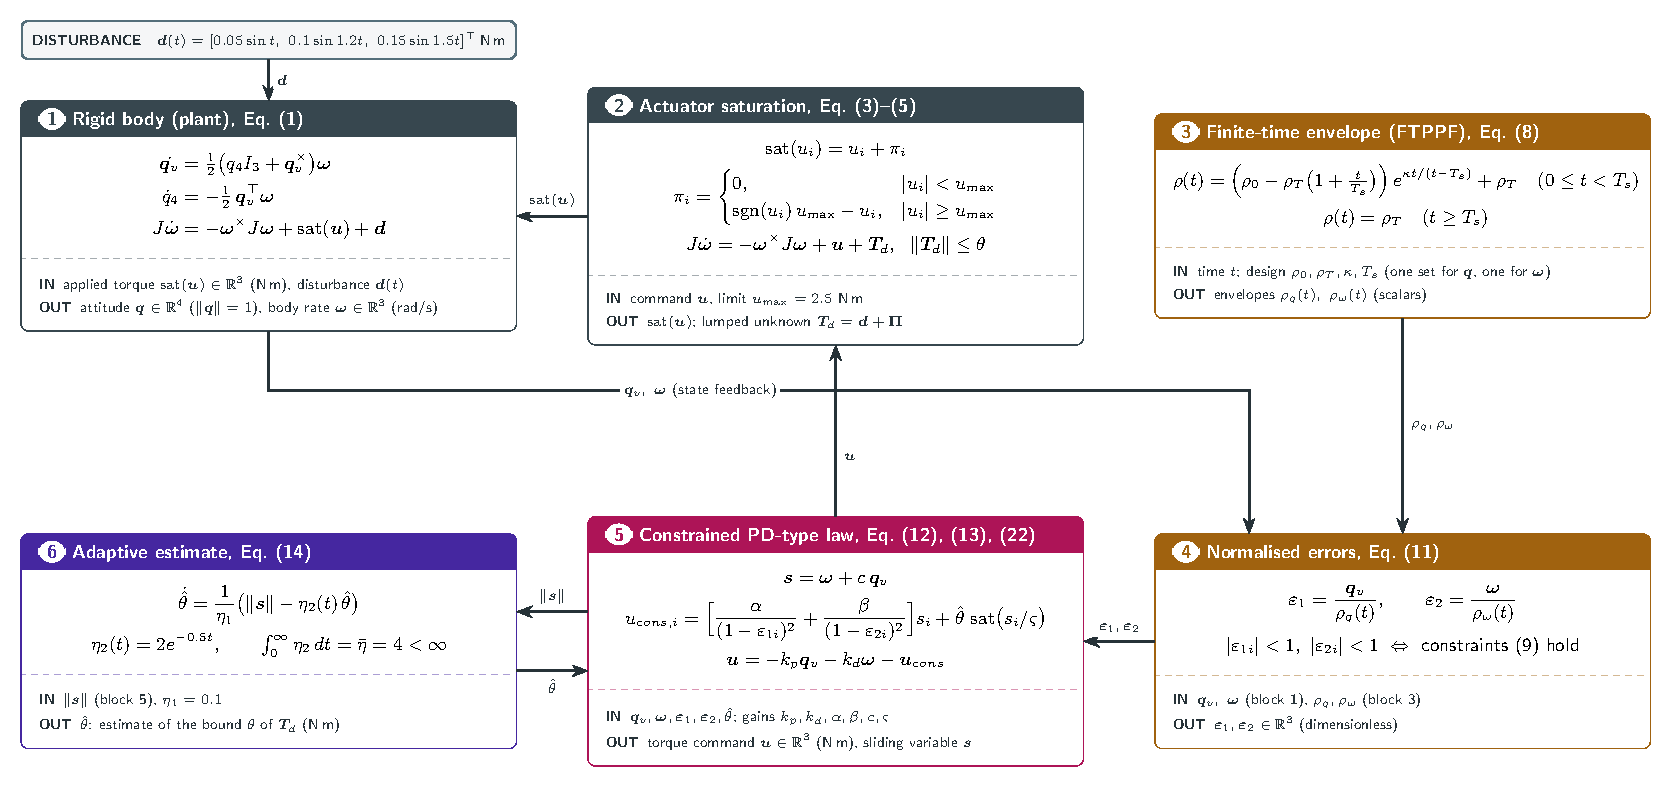
\includegraphics[width=\linewidth]{flow_paper.pdf}
\caption{Equation flow of the paper. Block numbers are used throughout this document.}
\label{fig:flowpaper}
\end{figure}

\subsection{Plant and saturation (blocks 1--2)}

\begin{eqbox}{cPlant}{Eq. (1), (3)--(5)}
\begin{gather*}
\dot\qv=\tfrac12(q_4I_3+\qv^\times)\vw,\qquad \dot q_4=-\tfrac12\qv^\top\vw,\qquad J\dot\vw=-\vw^\times J\vw+\sat(\vu)+\vd\\
\sat(u_i)=\sgn(u_i)\min(|u_i|,\umax)
\end{gather*}
\end{eqbox}
The simulator is written for a whole \emph{batch} of rigid bodies at once (rows of the arrays), which is what makes a
300-run Monte-Carlo study take seconds instead of hours.
\pyfile{107}{114}{\repro}{paper\_reproduction.py --- rhs(): Eq. (1) for a batch}

\subsection{Envelope (block 3)}

\begin{eqbox}{cEnv}{Eq. (8)}
\[
\rho(t)=\Big(\rho_0-\rho_T\big(1+\tfrac{t}{T_s}\big)\Big)\exp\Big(\frac{\kappa t}{t-T_s}\Big)+\rho_T\ \ (0\le t<T_s),\qquad \rho(t)=\rho_T\ \ (t\ge T_s)
\]
\end{eqbox}
\pyfile{78}{85}{\repro}{paper\_reproduction.py --- ftppf(): Eq. (8)}

\resfig{fig01_ppf_comparison.png}{0.8\linewidth}{The finite-time property (cf.\ paper Fig.~2): the FTPPF reaches
$\rho_T$ exactly at $T_s=8$\,s and stays there; the exponential PPF is still $1.67\,\rho_T$ at that time.}{fig:ppf}

\subsection{Normalised errors, control law and adaptation (blocks 4--6)}

\begin{eqbox}{cCtrl}{Eq. (11), (12), (22), (14)}
\begin{gather*}
\veps_1=\frac{\qv}{\rho_q},\qquad \veps_2=\frac{\vw}{\rho_\omega},\qquad \vs=\vw+c\qv,\qquad
\dot\that=\frac{\|\vs\|-\eta_2\that}{\eta_1}\\
u_i=-k_pq_i-k_d\omega_i-\Big(\Big[\frac{\alpha}{(1-\varepsilon_{1i})^2}+\frac{\beta}{(1-\varepsilon_{2i})^2}\Big]s_i+\that\sat(s_i/\varsigma)\Big)
\end{gather*}
\end{eqbox}
\pyfile{117}{140}{\repro}{paper\_reproduction.py --- control(): Eq. (11), (12), (22) and the two comparison controllers}

\subsection{One simulation step}

Per step of 1\,ms: compute the control from the current state, saturate it, update all metrics, integrate the plant
with RK4 holding the torque constant, re-normalise the quaternion, update $\that$.
\pyfile{160}{192}{\repro}{paper\_reproduction.py --- simulate(): the main loop}

\subsection{The barrier form: paper versus symmetric}
\label{sec:barrierform}

\begin{idea}[One-sided or two-sided?]
The paper writes the barrier as $\alpha(1-\varepsilon_{1i})^{-2}$. Read literally, this gain explodes when
$\varepsilon_{1i}\to+1$ but tends to $\alpha/4$ when $\varepsilon_{1i}\to-1$: it guards the upper wall of the tube far more
than the lower wall. The two-sided version $\alpha(1-\varepsilon_{1i}^2)^{-2}$ treats both walls alike. Our first browser
and Gazebo code used the two-sided version without saying so. We now treat the paper form as the reference and report
the symmetric form as a named variant in every table.
\end{idea}

\resfig{fig09_barrier_forms.png}{0.7\linewidth}{Barrier gain as a function of $\varepsilon$ for $\alpha=1.5$.}{fig:barrier}

\begin{toybox}[the same state, two forms]
Part-1 state at $t=0$, axis 3: $\varepsilon_{13}=-0.833$ (closest to its wall of the three axes). Paper form:
$1.5/(1+0.833)^2=0.446$, plus the rate part, $g_3=1.59$. Symmetric form: $1.5/(1-0.694)^2=16.0$, $g_3=17.3$. The paper form
gives the axis that is closest to the wall the \emph{smallest} gain. (MATLAB: \code{step2\_normalised\_error.m}.)
\end{toybox}

% =====================================================================
\section{Reproduction of the Paper's Simulations}
\label{sec:repro}
% =====================================================================

The paper validates its controller on a rigid spacecraft in two parts (its Section IV). We repeated both with the
paper's inertia, disturbance, actuator limit, gains, envelopes and initial states (Mathematical Models, Section 2.3).
The paper publishes plots only, so we compare the behaviour of the plots and, in addition, report the metrics of
\cref{sec:metrics}, which make the comparison checkable. All numbers: \code{docs/results/metrics.md}.

% ---------------------------------------------------------------------
\subsection{Part 1: effect of the settling time $T_s$}
\label{sec:part1}
% ---------------------------------------------------------------------

\textbf{Paper's claim.} The quaternion and the angular velocity stay inside $\pm\rho(t)$, the controller does not let the
trajectories touch the boundaries, a smaller $T_s$ gives faster convergence, and the torque stays within the limit.

\begin{figure}[H]
\centering
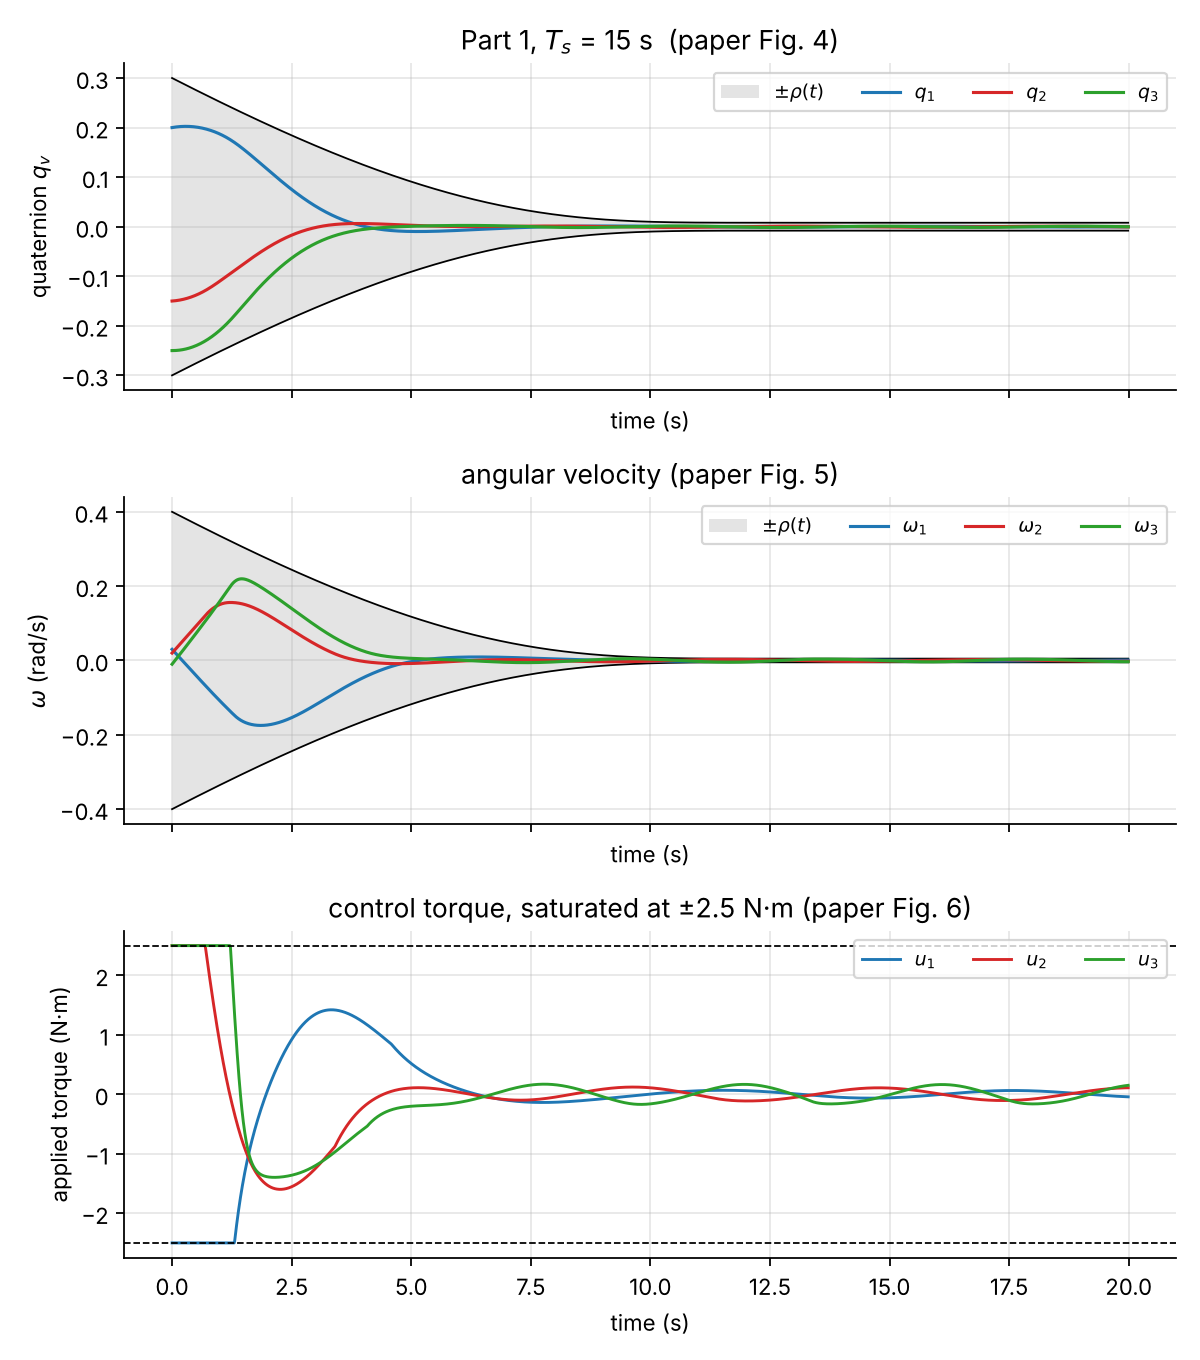
\includegraphics[width=0.49\linewidth]{fig02_part1_Ts15.png}\hfill
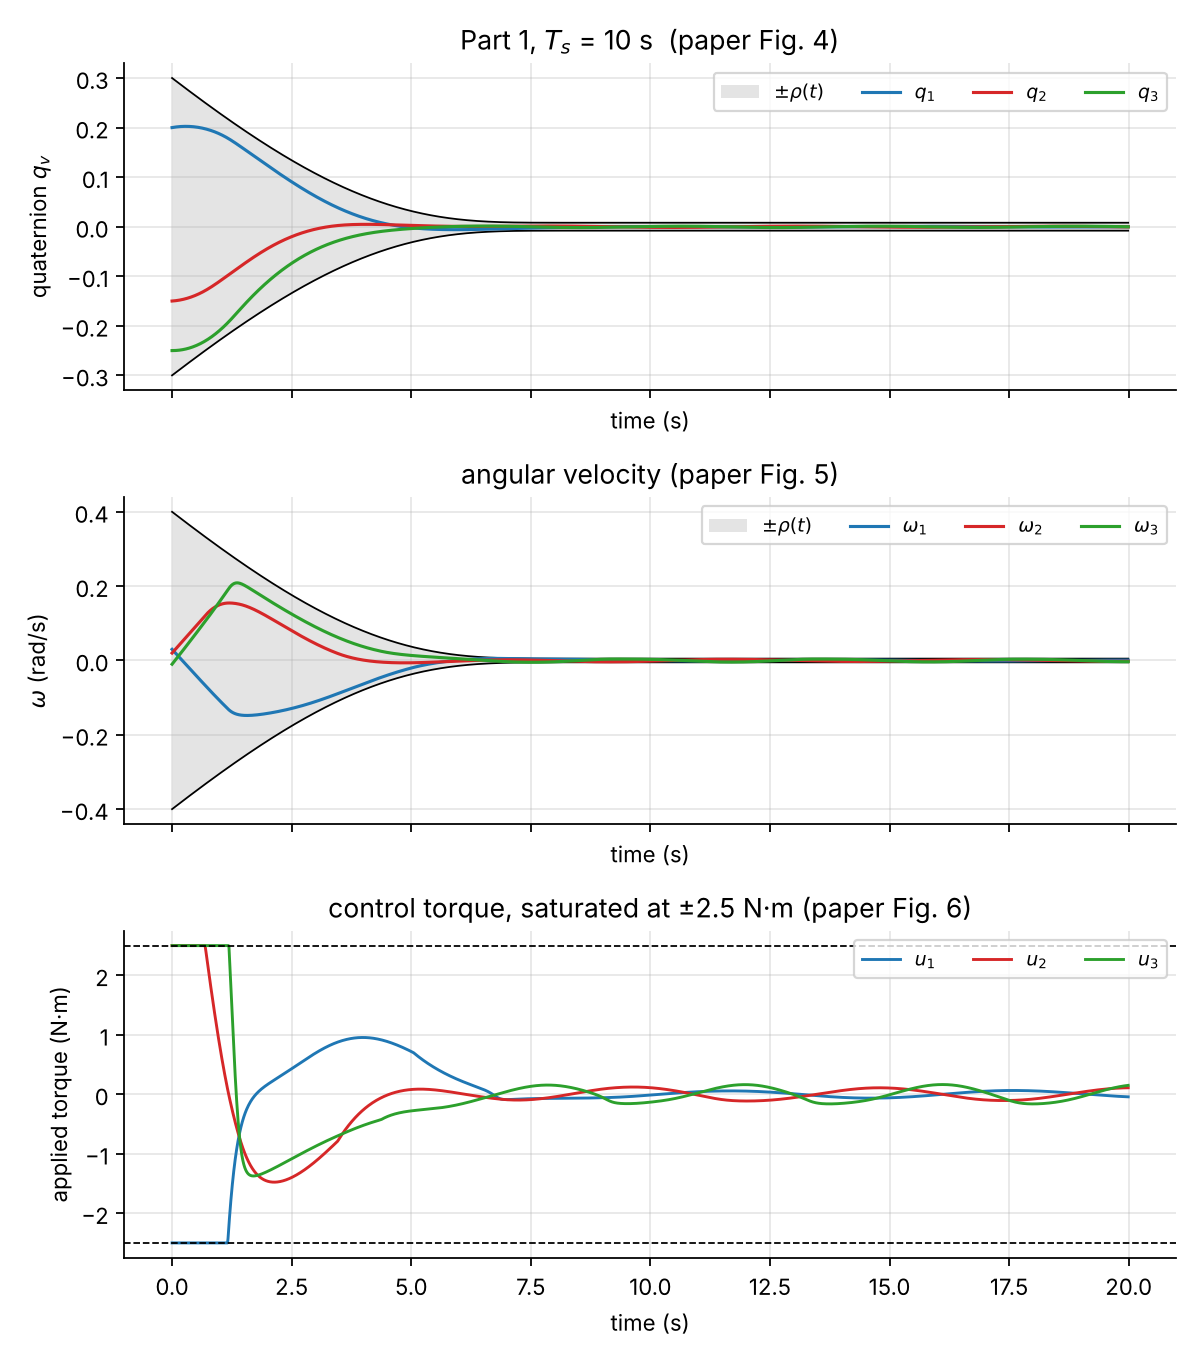
\includegraphics[width=0.49\linewidth]{fig02_part1_Ts10.png}
\caption{Part 1 reproduction, $T_s=15$\,s (left) and $T_s=10$\,s (right). Top: $\qv$ inside $\pm\rho_q$ (paper Fig.~4).
Middle: $\vw$ inside $\pm\rho_\omega$ (paper Fig.~5). Bottom: applied torque, saturated at $\pm2.5$\,N\,m during the first
second (paper Fig.~6).}
\label{fig:part1}
\end{figure}

\begin{table}[H]
\centering\small
\caption{Part 1 metrics (constrained law, paper form).}
\label{tab:part1}
\begin{tabular}{@{}lcc@{}}
\toprule
\textbf{Metric} & $T_s=15$\,s & $T_s=10$\,s\\
\midrule
time outside $\rho_q$ / outside $\rho_\omega$ & 0\,\% / 0\,\% & 0\,\% / 0\,\%\\
$\max|\varepsilon_1|$ / $\max|\varepsilon_2|$ & 0.871 / 0.912 & 0.924 / 0.942\\
settling time ($\|\qv\|<0.01$) & 5.25\,s & 4.53\,s\\
final $\|\qv\|$ / final $\|\vw\|$ (rad/s) & $4.4\times10^{-4}$ / $4.0\times10^{-3}$ & $4.5\times10^{-4}$ / $4.1\times10^{-3}$\\
time with commanded torque at the limit & 6.5\,\% & 5.9\,\%\\
peak commanded torque (before saturation) & 10.54\,N\,m & 10.54\,N\,m\\
$\that$ at 20\,s & 0.433 & 0.416\\
\bottomrule
\end{tabular}
\end{table}

\resfig{fig03_part1_convergence.png}{0.95\linewidth}{Convergence on a log scale: with $T_s=10$\,s both $\|\qv\|$ and $\|\vw\|$
fall faster during the transient. After the envelope has closed, both runs settle on the same small residual set by the
disturbance and the boundary layer.}{fig:part1conv}

\begin{projbox}[result]
Every statement of Part~1 is reproduced: 0\,\% of the time outside either envelope for both settling times, the largest
normalised error is 0.942 (6\,\% margin to the wall), the shorter $T_s$ settles 0.72\,s earlier, and the applied torque
never exceeds 2.5\,N\,m (it saturates only in the first $\approx1.2$\,s, when the initial error is largest). The peak of the
\emph{commanded} torque (10.54\,N\,m, at $t=0$) is the value computed by hand in the Mathematical Models (block 5).
\end{projbox}

% ---------------------------------------------------------------------
\subsection{Part 2: constrained PD-type versus conventional PD}
\label{sec:part2}
% ---------------------------------------------------------------------

\textbf{Paper's claim.} With the same maximum control torque, the constrained law keeps both states inside their
envelopes, whereas conventional PD is ``not capable of providing as fast and accurate convergence''.

\textbf{Set-up.} Both controllers have the same $k_p=40$, $k_d=20$, the same 2.5\,N\,m limit, the same disturbance and
the same initial state $\vq(0)=[0.3,-0.2,-0.3,0.8832]$, $\vw(0)=[-0.02,-0.02,0.025]$\,rad/s; conventional PD is the law
with $\vu_{cons}=0$. $T_s=15$\,s and $\rho_{q0}=0.36$ (the paper's 0.3 would put the initial state on the boundary).

\resfig{fig04_part2_quaternion.png}{0.92\linewidth}{Part 2, quaternion (paper Fig.~7). Both controllers keep $\qv$ inside
$\pm\rho_q$ in this run.}{fig:part2q}

\resfig{fig05_part2_angular_velocity.png}{0.92\linewidth}{Part 2, angular velocity (paper Fig.~8). Black dots: conventional
PD outside $\pm\rho_\omega$, both during the transient ($t\approx2$\,s, axes 1 and 3) and in steady state, where the
disturbance keeps $|\omega_3|$ above $\rho_{\omega T}=0.005$\,rad/s. The constrained law stays inside throughout.}{fig:part2w}

\resfig{fig06_part2_torque.png}{0.95\linewidth}{Part 2, applied torque (paper Fig.~9). Both controllers use the same maximum
torque, 2.5\,N\,m, as in the paper.}{fig:part2u}

\resfig{fig07_part2_normalised_error.png}{0.95\linewidth}{The clearest view of the constraint: $\max_i|\varepsilon_{1i}|$ and
$\max_i|\varepsilon_{2i}|$. Below the red line means inside. Conventional PD crosses it for the angular velocity.}{fig:part2eps}

\begin{table}[H]
\centering\small
\setlength{\tabcolsep}{3.5pt}
\caption{Part 2 metrics ($T_s=15$\,s, $\rho_{q0}=0.36$; same gains, limit, disturbance and initial state).}
\label{tab:part2}
\footnotesize
\begin{tabular}{@{}lccc@{}}
\toprule
\textbf{Metric} & \textbf{constrained (paper)} & \textbf{constrained (symm.)} & \textbf{conventional PD}\\
\midrule
time outside $\rho_q$ & 0\,\% & 0\,\% & 0\,\%\\
time outside $\rho_\omega$ & \textbf{0\,\%} & \textbf{0\,\%} & \textbf{27.5\,\%}\\
$\max|\varepsilon_1|$ / $\max|\varepsilon_2|$ & 0.868 / 0.904 & 0.868 / 0.837 & 0.868 / 1.496\\
time with commanded torque at the limit & 6.3\,\% & 7.2\,\% & 14.0\,\%\\
peak commanded torque & 18.8\,N\,m & 13.8\,N\,m & 11.6\,N\,m\\
settling time ($\|\qv\|<0.01$) & 5.79\,s & 4.19\,s & 6.31\,s\\
final $\|\vw\|$ (rad/s) & 0.0040 & 0.0040 & 0.0083\\
final $\|\qv\|$ & $4.4\times10^{-4}$ & $3.9\times10^{-4}$ & $9.0\times10^{-4}$\\
torque energy $\int\|\sat(\vu)\|^2dt$ & 38.9 & 41.5 & 60.5\\
final $\that$ & 0.439 & 0.435 & --\\
\bottomrule
\end{tabular}
\end{table}

\begin{projbox}[result]
The central claim of the paper is reproduced. At the same 2.5\,N\,m limit the constrained law keeps the angular velocity
inside its envelope all the time, conventional PD is outside 27.5\,\% of the time (peak $|\varepsilon_2|=1.50$). The
constrained law also settles earlier (5.79 vs.\ 6.31\,s), ends with half the rate error (0.0040 vs.\ 0.0083\,rad/s) and less
than half the attitude error, spends less than half as much time at the torque limit (6.3 vs.\ 14.0\,\%) and uses 36\,\%
less torque energy.
\end{projbox}

\begin{warn}[Reading Part 2 fairly]
In this run the conventional PD also keeps the \emph{quaternion} inside its envelope; the advantage of the constrained
law is in the angular velocity, the residual error and the control effort. The constrained law commands a higher
\emph{peak} torque (18.8\,N\,m) for an instant, but the actuator delivers at most 2.5\,N\,m to both, which is exactly the
paper's ``same maximum control effort''.
\end{warn}

\subsection{Adaptive estimate and Lyapunov function}

\resfig{fig08_theta_hat_and_lyapunov.png}{0.95\linewidth}{Left: $\that(t)$, Eq.~(14). It rises while $\|\vs\|$ is large, drops
when the leakage $\eta_2$ is still strong, and then creeps upwards because $\eta_2=2e^{-0.5t}$ has almost vanished while a
small residual $\|\vs\|$ remains (Mathematical Models, block 6). Right: the state part $V_x$ of the Lyapunov function (15) along the
Part~2 trajectory. It falls by five orders of magnitude within 9\,s and then stays near $10^{-4}$, a floor set by the
persistent disturbance and the boundary layer (ultimate boundedness rather than exact convergence; Mathematical
Models, Theorem~1). The $\ttil$ part of (15) cannot be plotted because the true bound $\theta$ is unknown.}{fig:theta}

% ---------------------------------------------------------------------
\subsection{Independent cross-check in MATLAB}
\label{sec:crosscheck}
% ---------------------------------------------------------------------

\code{toy\_model/step6\_spacecraft\_closed\_loop.m} is a second implementation of the same experiments in a different language, with its own RK4
integrator and its own control law (\code{lib/control\_law.m}); only the equations and parameters are shared.
% generated by docs/make_crosscheck.py - do not edit by hand
\cref{tab:crosscheck} compares the two implementations metric by metric.
\begin{table}[H]
\centering\small
\caption{Cross-check: Python (\code{paper\_reproduction.py}) vs.\ MATLAB (\code{toy\_model/step6}).}
\label{tab:crosscheck}
\begin{tabular}{@{}llcc@{}}
\toprule
\textbf{Case} & \textbf{Metric} & \textbf{Python} & \textbf{MATLAB}\\
\midrule
Part 1, $T_s=15$\,s & $\max|\varepsilon_1|$ & 0.871 & 0.871\\
 & $\max|\varepsilon_2|$ & 0.912 & 0.912\\
 & time outside $\rho_q$ (\%) & 0.0 & 0.0\\
 & time outside $\rho_\omega$ (\%) & 0.0 & 0.0\\
 & settling time (s) & 5.25 & 5.25\\
Part 1, $T_s=10$\,s & $\max|\varepsilon_1|$ & 0.924 & 0.924\\
 & $\max|\varepsilon_2|$ & 0.941 & 0.942\\
 & time outside $\rho_q$ (\%) & 0.0 & 0.0\\
 & time outside $\rho_\omega$ (\%) & 0.0 & 0.0\\
 & settling time (s) & 4.53 & 4.53\\
Part 2, paper form & $\max|\varepsilon_2|$ & 0.904 & 0.904\\
 & time outside $\rho_\omega$ (\%) & 0.0 & 0.0\\
 & time at torque limit (\%) & 6.3 & 6.3\\
 & settling time (s) & 5.79 & 5.79\\
 & torque energy & 38.9 & 38.9\\
Part 2, symmetric & $\max|\varepsilon_2|$ & 0.837 & 0.837\\
 & time outside $\rho_\omega$ (\%) & 0.0 & 0.0\\
 & time at torque limit (\%) & 7.2 & 7.2\\
 & settling time (s) & 4.19 & 4.19\\
 & torque energy & 41.5 & 41.5\\
Part 2, conv.\ PD & $\max|\varepsilon_2|$ & 1.496 & 1.496\\
 & time outside $\rho_\omega$ (\%) & 27.5 & 27.5\\
 & time at torque limit (\%) & 14.0 & 14.0\\
 & settling time (s) & 6.31 & 6.31\\
 & torque energy & 60.5 & 60.5\\
\bottomrule
\end{tabular}
\end{table}
The largest difference over all 25 entries is 0.001 (in the units of the metric).


% =====================================================================
\section{Beyond the Paper: Robustness, Sensitivity and Findings}
\label{sec:beyond}
% =====================================================================

The paper shows two single runs. To know whether its conclusions hold in general, and where they stop holding, we ran
three Monte-Carlo studies (300 runs each, the same random draws for all three controllers, fixed seed) and a
sensitivity study on the parameters the paper does not state.

% ---------------------------------------------------------------------
\subsection{Monte-Carlo studies}
\label{sec:mc}
% ---------------------------------------------------------------------

\begin{center}\small
\begin{tabularx}{\linewidth}{@{}l X@{}}
\toprule
\textbf{Study} & \textbf{Random draws (per run)}\\
\midrule
A --- paper regime & attitude uniform inside 90\,\% of the envelope ($|q_i(0)|\le0.9\rho_{q0}$), $|\omega_i(0)|\le0.05$\,rad/s, paper disturbance\\
B --- disturbance amplitude & as A, disturbance multiplied by a factor drawn from $U[0.5,\,3]$\\
C --- initial-rate stress & as A, but $|\omega_i(0)|$ up to $0.9\rho_{\omega0}=0.36$\,rad/s\\
\bottomrule
\end{tabularx}
\end{center}

\resfig{fig11_monte_carlo.png}{\linewidth}{Fraction of violation-free runs. A: paper regime with 95\,\% Wilson confidence
intervals. B: by disturbance scale. C: by initial rate.}{fig:mc}

\begin{table}[H]
\centering\small
\setlength{\tabcolsep}{3.5pt}
\caption{Monte-Carlo results ($N=300$ per controller and study). ``Violation-free'' = never outside either envelope.}
\label{tab:mc}
\begin{tabular}{@{}llcccc@{}}
\toprule
\textbf{Study} & \textbf{Controller} & \textbf{violation-free} & \textbf{95\,\% CI} & \textbf{median settling} & \textbf{mean torque energy}\\
\midrule
A & constrained (paper) & \textbf{97.0\,\%} & [94.4, 98.4] & 4.85\,s & 27.9\\
  & constrained (symmetric) & 97.7\,\% & [95.3, 98.9] & 4.89\,s & 28.5\\
  & conventional PD & 0.0\,\% & [0.0, 1.3] & 5.93\,s & 36.0\\
\midrule
B & constrained (paper) & 21.3\,\% & [17.1, 26.3] & 5.05\,s & 29.1\\
  & constrained (symmetric) & \textbf{97.3\,\%} & [94.8, 98.6] & 5.03\,s & 29.8\\
  & conventional PD & 3.0\,\% & [1.6, 5.6] & 6.00\,s & 37.2\\
\midrule
C & constrained (paper) & 50.3\,\% & [44.7, 56.0] & 6.72\,s & 76.5\\
  & constrained (symmetric) & 51.3\,\% & [45.7, 56.9] & 6.68\,s & 89.6\\
  & conventional PD & 0.0\,\% & [0.0, 1.3] & 7.65\,s & 59.3\\
\bottomrule
\end{tabular}
\end{table}

\begin{projbox}[what the three studies say]
\begin{enumerate}[leftmargin=*]
  \item \textbf{A confirms the paper in general, not just for its two initial states.} In the paper's operating regime
        97\,\% of all random starts stay inside both envelopes with the paper's law; conventional PD fails in every run
        (it leaves the rate envelope both during the transient and after it has closed to $\rho_{\omega T}=0.005$\,rad/s,
        where the disturbance keeps its residual rate too large). The
        constrained law also settles about 1\,s earlier and uses 22\,\% less torque energy on average.
  \item \textbf{B: the paper's one-sided barrier is sensitive to the disturbance size; the symmetric barrier is not.} Up to
        the paper's disturbance amplitude every form works (100\,\% for both constrained forms in the $0.5$--$1\times$ bin).
        Above it, the paper form drops to 23\,\% ($1$--$1.5\times$) and 0\,\% beyond $1.5\times$, while the symmetric form stays at
        96--97\,\% up to $3\times$. In the runs above $1.5\times$, \emph{every} sample outside the envelope is at the \emph{lower} wall of the rate
        envelope ($\omega_i<-\rho_\omega$), and all of them occur late ($t>11$\,s, when the tube is narrow), where the paper's barrier
        gain stays near $\beta/4$: exactly the one-sided property of \cref{sec:barrierform}.
  \item \textbf{C: no controller can beat physics.} With $J\approx17$\,kg\,m$^2$ and 2.5\,N\,m the body can decelerate by only
        about $0.15$\,rad/s$^2$ (Mathematical Models, block 1). An initial rate of 0.3\,rad/s needs about 2\,s to stop, while
        the rate envelope is already closing. Both constrained forms degrade identically with the initial rate (100\,\%
        below 0.12\,rad/s, about 35\,\% at 0.33\,rad/s): this is a feasibility limit of the envelope, not a controller defect.
\end{enumerate}
\end{projbox}

% ---------------------------------------------------------------------
\subsection{Sensitivity to the parameters the paper does not give}
\label{sec:sens}
% ---------------------------------------------------------------------

\begin{table}[H]
\centering\small
\caption{Constrained law (paper form), Part-2 initial state, different $T_s$ and $\rho_{q0}$.}
\label{tab:sens}
\begin{tabular}{@{}cccccc@{}}
\toprule
$T_s$ (s) & $\rho_{q0}$ & outside $\rho_q$ & outside $\rho_\omega$ & torque at limit & $\max|\varepsilon_1|$\\
\midrule
15 & 0.36 (ours) & 0.0\,\% & 0.0\,\% & 6.3\,\% & 0.868\\
15 & 0.50 & 0.0\,\% & 0.0\,\% & 7.7\,\% & 0.625\\
10 & 0.50 & 0.0\,\% & 9.6\,\% & 7.4\,\% & 0.813\\
10 & 0.36 & 65.9\,\% & 55.8\,\% & 71.3\,\% & 6.554\\
\bottomrule
\end{tabular}
\end{table}

\resfig{fig10_infeasible_envelope.png}{0.95\linewidth}{An infeasible envelope ($T_s=10$\,s with the tight $\rho_{q0}=0.36$, Part-2
state): the barrier asks for more torque than 2.5\,N\,m, the torque stays pinned at the limit and the constraint is
lost.}{fig:infeasible}

\begin{warn}[Lesson: the envelope must be feasible for the actuator]
The paper presents $\rho_0$, $\rho_T$, $T_s$ as free design choices ``based on the requirements''. They are not
independent of $\umax$: if the tube closes faster than the saturated actuator can turn the body, no gain can keep the state
inside, and the barrier only drives the actuator into permanent saturation. This is the same limit as Monte-Carlo C, and it
is the main design rule we took to the X3, whose inertia and torque authority are completely different.
\end{warn}

% ---------------------------------------------------------------------
\subsection{Findings: what the paper does not say}
\label{sec:findings}
% ---------------------------------------------------------------------

\begin{center}\small
\begin{longtable}{@{}l p{6.4cm} p{6.6cm}@{}}
\toprule
\textbf{\#} & \textbf{Finding} & \textbf{How we handled it}\\
\midrule\endhead
P1 & Four values are not given: $c$, $\varsigma$, the Part-2 settling time and a usable Part-2 $\rho_{q0}$. & $c=0.5$ (satisfies Theorem 1, $c<0.964$), $\varsigma=0.02$, $T_s=15$\,s, $\rho_{q0}=0.36$; sensitivity measured (\cref{tab:sens}).\\
P2 & Part 2 starts on its own boundary ($|q_1(0)|=|q_3(0)|=0.3=\rho_{q0}$), so $(1-\varepsilon)^{-2}=\infty$ and Remark~7 is violated. & $\rho_{q0}=1.2\max|q_i(0)|=0.36$.\\
P3 & The barrier $(1-\varepsilon)^{-2}$ is one-sided. & Paper form is the reference; the symmetric form is reported as a variant; Monte-Carlo B shows the difference.\\
P4 & Envelope parameters must be feasible for $\umax$ and $J$. & Sensitivity study and Monte-Carlo C; used to size the X3 envelope.\\
P5 & Theorem 1 proves convergence to the origin, not that $|\varepsilon|<1$ for all $t$. & Constraint satisfaction is reported as measured, never as guaranteed.\\
P6 & Eq.~(15) is printed with $(1-q_0^2)$ and $\ttil^2/\eta_1$; the derivative (17) follows from $(1-q_0)^2$ and $\tfrac{\eta_1}{2}\ttil^2$. & Written in the consistent form (Mathematical Models, Theorem 1).\\
P7 & With the boundary layer (22) and a leakage that vanishes, $\that$ slowly drifts upward. & Observed (\cref{fig:theta}); on the X3 the leakage has a floor and $\that$ an upper bound.\\
\bottomrule
\end{longtable}
\end{center}

% =====================================================================
\section{Putting the Controller on the Gazebo X3 Quadcopter}
\label{sec:x3}
% =====================================================================

\subsection{Architecture}

\begin{figure}[H]
\centering
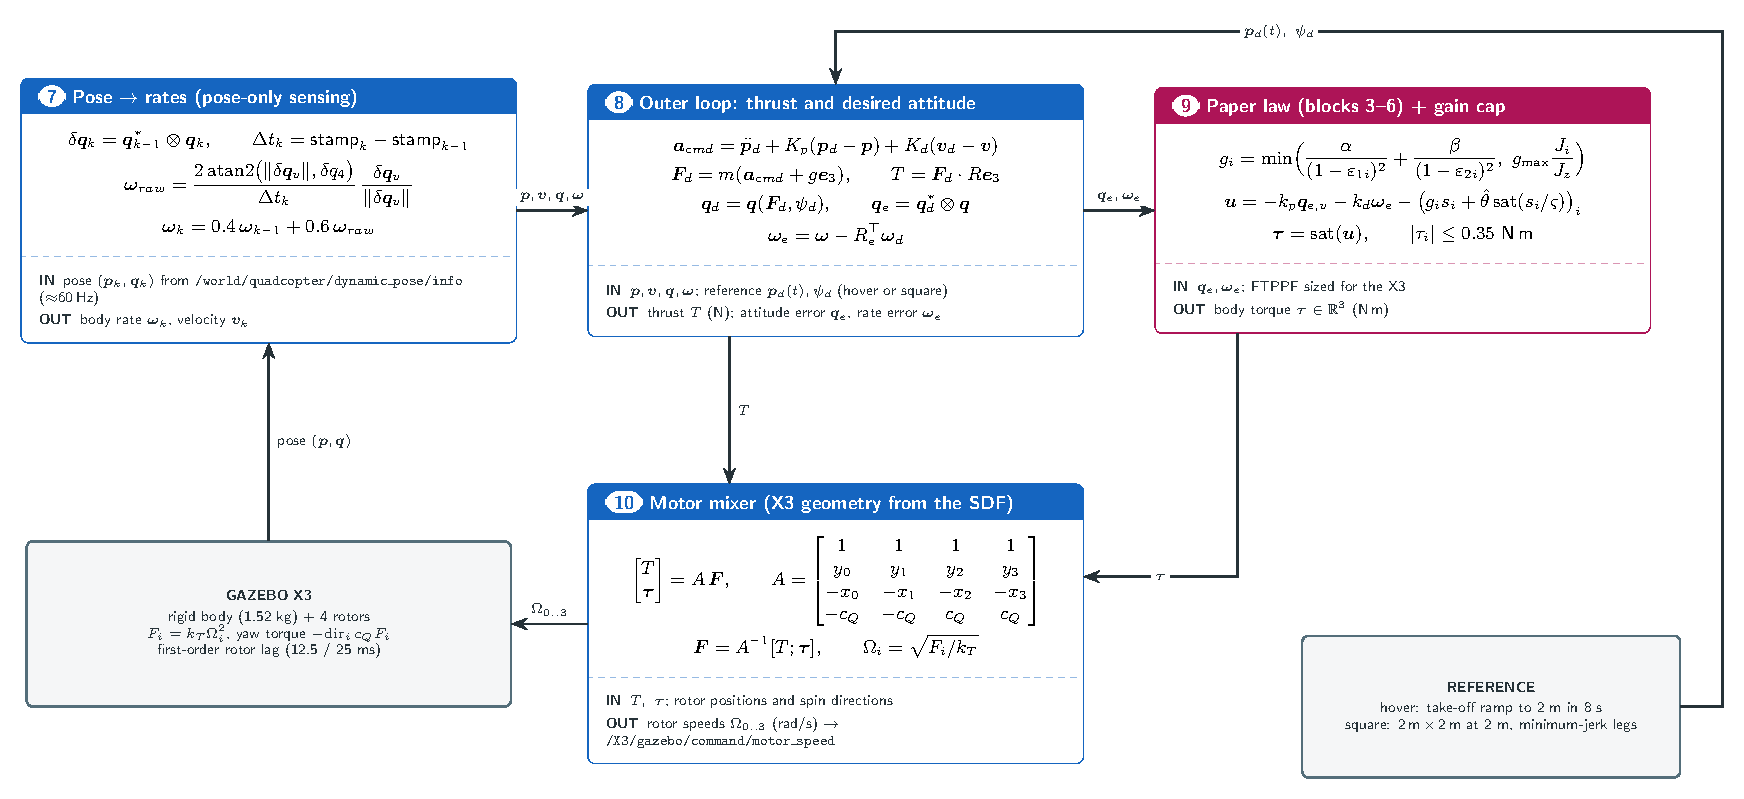
\includegraphics[width=\linewidth]{flow_x3.pdf}
\caption{Implementation flow on the X3 (Mathematical Models, Section 4). Blocks 3--6 of the paper sit inside block 9.}
\label{fig:flowx3}
\end{figure}

\begin{center}\small
\begin{tabularx}{\linewidth}{@{}l l X@{}}
\toprule
\textbf{Topic} & \textbf{Type} & \textbf{Use}\\
\midrule
\code{/world/quadcopter/dynamic\_pose/info} & \code{geometry\_msgs/PoseArray} & input: pose of the X3 with the simulation time stamp ($\approx$60\,Hz)\\
\code{/X3/gazebo/command/motor\_speed} & \code{actuator\_msgs/Actuators} & output: four rotor speeds in rad/s\\
\bottomrule
\end{tabularx}
\end{center}

\textbf{Why a software-in-the-loop surrogate.} Diagnosing a crash inside Gazebo is slow: one run per minute, no access to
the internal state, no exact repetition. We therefore wrote \code{x3\_sim/x3\_model.py}, a model of the same vehicle in
which \emph{every constant is copied from the Gazebo model files} (mass, inertia, rotor positions and spin directions,
thrust and moment constants, rotor time constants and speed limit, rotor drag), integrated with RK4 at 1\,ms, sampled at
the Gazebo pose rate of 60\,Hz with one sample of transport delay. The controller sees only what the ROS node sees: a
time stamp, a position and a quaternion. Both controllers are plain classes with the same \code{update(stamp, p, q)}
interface, so the identical code runs in the surrogate, in the offline test and inside \code{gazebo.py}.

\begin{warn}[What the surrogate does not model]
Rotor gyroscopic effects (rotor inertia is about 0.1\,\% of the body's), blade flapping, contacts other than a flat ground,
sensor noise and the ROS/Gazebo transport beyond a fixed delay. Results on the surrogate are therefore ``best case'' for
noise; Gazebo logs processed with \code{plot\_gazebo\_log.py} use the same metric definitions so the two can be compared
line by line.
\end{warn}

% ---------------------------------------------------------------------
\subsection{Why the first Gazebo node crashed}
\label{sec:x3fault}
% ---------------------------------------------------------------------

Our first node (\code{legacy/gazebo\_v1.py}) made the X3 take off and climb, then lose its attitude and crash. To find out
why without guessing, \code{OriginalGazeboController} is a line-by-line port of that node's control logic (only the ROS
plumbing removed). On the surrogate it reproduces the observed behaviour, and each suspected fault can be switched off on
its own (experiment E1).

\begin{center}\small
\begin{longtable}{@{}l p{6.0cm} p{6.6cm}@{}}
\toprule
\textbf{\#} & \textbf{Fault in v1} & \textbf{Consequence / fix in v2}\\
\midrule\endhead
F9 & Mixer signs taken from a generic ``+/$-$'' template that does not match the X3 rotor numbering. & A pitch command produced roll torque ($-0.93$ per unit), nothing produced pitch torque (\cref{tab:mixer}). Fix: exact inverse of the allocation matrix built from the SDF (block 10).\\
F10 & Yaw term divided by $c_Q$ instead of $k_Tc_Q$. & Yaw authority $10^{5}$ times too small, yaw uncontrolled. Fix: same allocation matrix.\\
F14 & \code{last\_z} set once at start and never updated. & ``Vertical speed'' $=(z-z_0)/\Delta t$ grows with height, the altitude loop cuts thrust: the drone hops and falls. Fix: update every sample.\\
F11 & Body rate from $2(\vq_k-\vq_{k-1})_v/\Delta t$ with a 0.10 filter. & Wrong axes when yawed, $\approx$150\,ms lag; slow limit cycle. Fix: $\vq_{k-1}^*\otimes\vq_k$, filter 0.6 (block 7).\\
F12 & $\Delta t$ from the wall clock (\code{time.time()}). & Timing does not match simulation time when Gazebo runs slower or faster than real time. Fix: message stamp.\\
F13 & Attitude error = raw world quaternion. & Works only for yaw 0 and no position control. Fix: $\vq_e=\vq_d^*\otimes\vq$ with an outer position loop (block 8).\\
F3 & Envelope effectively inactive ($\rho_{q0}=2$ although $|q_i|\le1$; $\alpha=\beta=0.01$; $\vu_{cons}$ clipped to 0.05\,N\,m). & The first node was in practice a plain PD. Fix: envelope and gains sized for the X3 (block 9).\\
F15 & (new in v2) unbounded barrier gain on a 60\,Hz delayed loop. & Cap $g_i\le J_i/J_z$ (block 9; MATLAB step 8).\\
\bottomrule
\end{longtable}
\end{center}

\begin{table}[H]
\centering\small
\caption{Torque produced on the X3 per unit torque commanded by the v1 mixer (ideal: identity).}
\label{tab:mixer}
\begin{tabular}{@{}lccc@{}}
\toprule
& cmd $\tau_x$ & cmd $\tau_y$ & cmd $\tau_z$\\
\midrule
produced $\tau_x$ & $+0.044$ & $\mathbf{-0.933}$ & $0$\\
produced $\tau_y$ & $0$ & $\mathbf{0}$ & $7\times10^{-5}$\\
produced $\tau_z$ & $+0.071$ & $0$ & $\mathbf{0}$\\
\bottomrule
\end{tabular}
\end{table}

The two faults in the port of v1 that matter most, next to their fixes:
\pyfile{70}{82}{\xctrl}{x3\_sim/controllers.py --- OriginalGazeboController (port of v1): z-rate and body rate}
\pyfile{113}{121}{\xctrl}{x3\_sim/controllers.py --- OriginalGazeboController (port of v1): the mixer}

\subsection{The corrected controller (v2)}

\code{FixedController} keeps the paper's law (Eq.~8, 11--14, 22) and adds blocks 7, 8, 10 and the gain cap of block 9.
\pyfile{215}{223}{\xctrl}{x3\_sim/controllers.py --- block 7: exact body rate (F11)}
\pyfile{264}{284}{\xctrl}{x3\_sim/controllers.py --- block 9: paper law with the sampled-data gain cap}
\pyfile{288}{310}{\xctrl}{x3\_sim/controllers.py --- block 10: allocation with thrust-priority de-saturation (F9, F10)}

\begin{table}[H]
\centering\small
\caption{Parameters of the paper's law: spacecraft (paper) and X3 (ours).}
\label{tab:x3params}
\begin{tabular}{@{}lcc@{}}
\toprule
\textbf{Parameter} & \textbf{Paper (spacecraft)} & \textbf{X3}\\
\midrule
inertia & $J\approx14$--$21$\,kg\,m$^2$ & $\diag(0.036,\,0.070,\,0.099)$\,kg\,m$^2$\\
torque limit & 2.5\,N\,m & 0.35\,N\,m (and rotor limits)\\
$k_p$, $k_d$ & 40, 20 & 4, 0.4\\
$\alpha$, $\beta$, $c$ & 1.5, 1.2, 0.5 & 0.15, 0.12, 1.0\\
$\eta_1$, $\eta_2$ & 0.1, $2e^{-0.5t}$ & 5, $\max(2e^{-0.5t},0.2)$, $\that\le0.1$\\
$\varsigma$ & 0.02 & 0.5\\
$\rho_q$: $\rho_0\to\rho_T$ & $0.3\to0.008$ & $0.30\to0.02$\\
$\rho_\omega$: $\rho_0\to\rho_T$ & $0.4\to0.005$\,rad/s & $2.5\to0.05$\,rad/s\\
$\kappa$, $T_s$ & 2.5, 10--15\,s & 2, 10\,s\\
natural frequency, damping (PD part) & 1.08\,rad/s, 0.54 & 7.5\,rad/s, 0.75 (roll)\\
barrier gain cap & none & $g_i\le J_i/J_z$ (0.36, 0.71, 1.0)\\
\bottomrule
\end{tabular}
\end{table}

\subsection{The ROS~2 node}

\code{gazebo.py} (v2) is a thin wrapper: it reads the pose and the \emph{message stamp}, calls the
\code{update()} method of \code{FixedController}, publishes the four rotor speeds, optionally injects the paper's disturbance as an extra
body torque through the rotors, logs everything and stops after the chosen duration. The experiment, controller and
disturbance are ROS parameters (\cref{sec:setup}). The offline test drives the real node file, with \code{rclpy} and the
two message types replaced by minimal stand-ins, against the surrogate at 60\,Hz with one sample of delay.

\begin{projbox}[offline test of the node (\code{tests/test\_gazebo\_node\_offline.py})]
Hover, 40\,s: final position $(0.000,\ 0.000,\ 2.000)$\,m. Square, 45\,s: returns to $(0.000,\ 0.000,\ 2.000)$\,m. Hover with
$0.5\times$ the paper's disturbance injected through the rotors (symmetric barrier): final position $(0.030,\ 0.056,\ 2.000)$\,m.
The log is processed by \code{plot\_gazebo\_log.py} without error. Result: \code{ALL OFFLINE NODE TESTS PASSED}.
\end{projbox}

% =====================================================================
\section{Results on the X3}
\label{sec:x3res}
% =====================================================================

All experiments run on the X3 surrogate (\cref{sec:x3}) at 60\,Hz with one sample of delay, with a tiny asymmetric
torque of $2\times10^{-4}$\,N\,m always applied so that a perfectly symmetric simulation cannot hide an instability.
Numbers: \code{docs/results/x3\_metrics.md}; script: \code{x3\_sim/run\_x3\_experiments.py}.

\begin{center}\small
\begin{tabularx}{\linewidth}{@{}l X@{}}
\toprule
\textbf{Exp.} & \textbf{Question}\\
\midrule
E0/E1 & Does the port of v1 crash like Gazebo did, and which fault causes it?\\
E2 & Does the corrected paper controller hover for 180\,s inside its envelopes?\\
E3 & With the paper's disturbance (scaled to what the X3 can produce), constrained vs.\ conventional PD?\\
E3b & What happens at the full paper disturbance?\\
E4 & Can it track a trajectory (2\,m\,$\times$\,2\,m square at 2\,m)?\\
E5 & How sensitive is it to control rate, delay and time-stamp jitter?\\
\bottomrule
\end{tabularx}
\end{center}

% ---------------------------------------------------------------------
\subsection{E0/E1: the crash of v1, reproduced and explained}
% ---------------------------------------------------------------------

\resfig{x3_E1_fault_isolation.png}{\linewidth}{Fault isolation: v1 with each fix switched on separately (60\,s, $\times$ = crash).}{fig:e1}

\begin{table}[H]
\centering\small
\caption{E1 fault isolation (60\,Hz).}
\label{tab:e1}
\begin{tabular}{@{}lcccc@{}}
\toprule
\textbf{Variant} & \textbf{crashed} & \textbf{crash time} & \textbf{max altitude} & \textbf{RMS tilt after 20\,s}\\
\midrule
v1 as is & yes & 5.07\,s & 0.24\,m & --\\
v1 + z-rate fix & yes & 5.68\,s & 1.06\,m & --\\
v1 + mixer fix & yes & 5.07\,s & 0.24\,m & --\\
v1 + mixer + z-rate fixes & no & -- & 2.00\,m & $2.03^\circ$\\
v1 + mixer + z-rate + body-rate fixes & no & -- & 1.97\,m & $0.007^\circ$\\
v1 as is at 250\,Hz & yes & 14.67\,s & 0.15\,m & --\\
\bottomrule
\end{tabular}
\end{table}

\resfig{x3_E0_v1_failure.png}{\linewidth}{v1 with only the z-rate fixed: the behaviour we saw in Gazebo. It climbs, then the
attitude diverges because pitch has no authority, the commanded roll torque saturates, and the vehicle crashes at 5.7\,s.}{fig:e0}

\begin{projbox}[conclusion of E1]
Two faults are each sufficient to crash the vehicle: the altitude-rate bug F14 (it never climbs above 0.24\,m) and the
mixer F9 (with F14 fixed it climbs to 1.06\,m and then tips over, exactly as observed in Gazebo). Fixing both gives a
stable flight; the remaining slow attitude limit cycle ($2^\circ$ RMS) comes from the lagging body-rate estimate F11 and
disappears with the exact estimate. A faster loop (250\,Hz) does not save v1: the faults are structural, not a matter of
rate.
\end{projbox}

% ---------------------------------------------------------------------
\subsection{E2: 180\,s hover with the paper's law}
% ---------------------------------------------------------------------

\resfig{x3_E2_hover_180s.png}{\linewidth}{E2, corrected controller (paper barrier form), 180\,s: altitude, horizontal position,
attitude error and body rate inside their envelopes, rotor commands and $\that$.}{fig:e2}

\begin{table}[H]
\centering\small
\caption{E2 metrics (after the 8\,s take-off ramp where stated).}
\label{tab:e2}
\begin{tabular}{@{}lc@{\hspace{1.5cm}}lc@{}}
\toprule
\textbf{Metric} & \textbf{Value} & \textbf{Metric} & \textbf{Value}\\
\midrule
crashed & no & time outside $\rho_q$ / $\rho_\omega$ & 0\,\% / 0\,\%\\
altitude RMS error ($t\ge10$\,s) & 0.02\,mm & $\max|\varepsilon_1|$ / $\max|\varepsilon_2|$ & 0.0023 / 0.0048\\
altitude max error ($t\ge10$\,s) & 0.24\,mm & mixer saturated & 0\,\% of the time\\
horizontal drift (max) & 0.21\,mm & rotor speeds ($t\ge10$\,s) & 659.9--660.7\,rad/s\\
tilt RMS ($t\ge10$\,s) & $0.003^\circ$ & $\that$ at 180\,s & 0.0012\,N\,m\\
\bottomrule
\end{tabular}
\end{table}

\begin{warn}[How to read these very small numbers]
The surrogate has no sensor noise and only the tiny test torque, so these are the errors of the control loop itself
(it is stable, well damped and has no limit cycle), not predictions of the errors in Gazebo or on hardware. The rotor
speeds sit at the hover value $660.4$\,rad/s computed by hand in the Mathematical Models (block 10).
\end{warn}

% ---------------------------------------------------------------------
\subsection{E3: disturbance rejection, constrained vs.\ conventional PD}
% ---------------------------------------------------------------------

The paper's disturbance has a yaw amplitude of 0.15\,N\,m, while the X3 can produce at most 0.106\,N\,m of yaw torque at
hover. E3 therefore uses $0.5\times$ the paper's $\vd(t)$, applied from $t=15$\,s to 180\,s (E3b uses $1\times$).

\resfig{x3_E3_disturbance_rates.png}{\linewidth}{E3, body rates against the rate envelope ($\rho_{\omega T}=0.05$\,rad/s), first
60\,s. Black: outside. The paper form touches the \emph{lower} yaw wall, the symmetric form never leaves, conventional PD
leaves at both walls on every yaw oscillation.}{fig:e3}

\resfig{x3_E3_violation_bars.png}{0.8\linewidth}{E3, percentage of time outside each envelope (15--180\,s).}{fig:e3bars}

\begin{table}[H]
\centering\small
\caption{E3 metrics, disturbance $0.5\times$ paper $\vd(t)$, $t=15$--$180$\,s.}
\label{tab:e3}
\begin{tabular}{@{}lccc@{}}
\toprule
\textbf{Metric} & \textbf{constrained (paper)} & \textbf{constrained (symm.)} & \textbf{conventional PD}\\
\midrule
crashed & no & no & no\\
time outside $\rho_q$ & 0\,\% & 0\,\% & 0.16\,\%\\
time outside $\rho_\omega$ & 6.0\,\% & \textbf{0\,\%} & 36.4\,\%\\
$\max|\varepsilon_1|$ / $\max|\varepsilon_2|$ & 0.93 / 1.21 & 0.72 / 0.77 & 1.02 / 1.25\\
tilt RMS & $0.43^\circ$ & $0.43^\circ$ & $0.52^\circ$\\
yaw RMS & $1.16^\circ$ & $1.06^\circ$ & $1.61^\circ$\\
max horizontal error & 12.3\,cm & 13.1\,cm & 14.9\,cm\\
\bottomrule
\end{tabular}
\end{table}

\begin{projbox}[conclusion of E3]
On the quadcopter the paper's qualitative claim holds again: with the same gains and limits, the constrained law cuts the
time outside the rate envelope from 36.4\,\% (PD) to 6.0\,\% (paper form) and to 0\,\% (symmetric form), and reduces the tilt
and yaw errors. The paper form's remaining violations are all at the lower yaw wall, the one-sided effect seen in the
spacecraft Monte-Carlo study B.
\end{projbox}

\begin{warn}[E3b: full paper disturbance]
At $1\times$ the paper's disturbance the yaw torque demanded exceeds what the X3's rotors can produce while hovering
(0.15 vs.\ 0.106\,N\,m): the mixer is saturated 97\,\% of the time and all three controllers are outside the envelopes
96--98\,\% of the time (none crashes; thrust has priority). This is the feasibility limit of \cref{sec:sens} in physical form:
no controller can satisfy a constraint the actuators cannot.
\end{warn}

% ---------------------------------------------------------------------
\subsection{E4: square trajectory}
% ---------------------------------------------------------------------

\resfig{x3_E4_square_trajectory.png}{\linewidth}{E4, $2\times2$\,m square at 2\,m altitude with minimum-jerk legs of 5\,s and 2\,s
holds. Left: 3-D path; middle: top view; right: position error (the first second is the take-off from the ground).}{fig:e4}

\begin{table}[H]
\centering\small
\caption{E4 metrics (after the take-off, $t\ge12$\,s).}
\label{tab:e4}
\begin{tabular}{@{}lcc@{}}
\toprule
\textbf{Metric} & \textbf{constrained (paper)} & \textbf{conventional PD}\\
\midrule
crashed & no & no\\
RMS / max position error & 4.03 / 7.90\,cm & 4.02 / 7.99\,cm\\
time outside $\rho_q$ & 0\,\% & 0\,\%\\
time outside $\rho_\omega$ & 4.7\,\% & 8.1\,\%\\
$\max|\varepsilon_1|$ & 0.30 & 0.36\\
\bottomrule
\end{tabular}
\end{table}

\begin{projbox}[conclusion of E4]
The paper's attitude law, with our outer loop, flies the square with 4\,cm RMS error and never leaves the attitude
envelope. Position tracking is set by the outer loop and is the same for both controllers. During the turns at the
corners the required roll and pitch rates exceed the hover-sized rate envelope ($\rho_{\omega T}=0.05$\,rad/s): the
constrained law halves the time outside it (4.7 vs.\ 8.1\,\%) but cannot remove it. For trajectory flight the rate envelope
should be widened to the rates the trajectory needs (feasibility again).
\end{projbox}

% ---------------------------------------------------------------------
\subsection{E5: control rate, delay and jitter}
% ---------------------------------------------------------------------

\begin{table}[H]
\centering\small
\caption{E5, disturbance $0.5\times$, 90\,s; time outside $\rho_q$ / $\rho_\omega$ in \%. No run crashed.}
\label{tab:e5}
\begin{tabular}{@{}lccc@{}}
\toprule
\textbf{Loop} & \textbf{constrained (paper)} & \textbf{constrained (symm.)} & \textbf{conventional PD}\\
\midrule
60\,Hz, 1 sample delay (nominal) & 0.0 / 6.6 & 0.0 / 0.0 & 0.4 / 36.2\\
100\,Hz, 1 sample delay & 0.0 / 6.8 & 0.0 / 0.0 & 0.4 / 36.7\\
250\,Hz, 1 sample delay & 0.0 / 7.1 & 0.0 / 0.0 & 1.5 / 36.9\\
60\,Hz, 2 samples delay & 18.0 / 90.6 & 20.7 / 90.6 & 0.4 / 36.3\\
60\,Hz, 2\,ms stamp jitter & 0.0 / 21.6 & 0.0 / 50.2 & 0.3 / 44.3\\
30\,Hz, 1 sample delay & 52.8 / 96.9 & 94.2 / 99.8 & 68.5 / 99.2\\
\bottomrule
\end{tabular}
\end{table}

\begin{warn}[What E5 tells us about deployment]
At 60\,Hz and faster the result is unchanged. Two things degrade the constrained laws far more than plain PD: a second
sample of delay (rate-envelope violations rise from 6.6 to 90.6\,\% for the paper form, while PD stays at 36\,\%) and
2\,ms of jitter on the time stamps (6.6 to 21.6\,\% for the paper form, 0 to 50.2\,\% for the symmetric form, 36 to 44\,\%
for PD). Both act through the body-rate estimate, which the barrier amplifies near the wall (even with the cap). At 30\,Hz no controller keeps the envelopes. In Gazebo the stamp must therefore be the simulation
time of the message (F12), and the pose rate should be at least 60\,Hz.
\end{warn}

% =====================================================================
\section{Visual Demonstrations (MuJoCo and Browser)}
\label{sec:demos}
% =====================================================================

These demos make the controller \emph{visible}; the quantitative evidence is in \cref{sec:repro,sec:beyond,sec:x3res}.

\subsection{MuJoCo: two bodies side by side}

\code{Drones\_Mujoco\_Pointing\_Trial.ipynb} integrates the paper's equations for two rigid bodies in MuJoCo's 3-D viewer:
the left (blue) one runs the constrained PD-type law (paper barrier form), the right (orange) one conventional PD. Three
demos are included: the paper's Part~2 manoeuvre, turning to any attitude entered as roll/pitch/yaw, and pointing the nose
at a target position (each body's dotted line of sight reaches the gold target only when it is truly aimed at it). The
notebook sizes $\rho_{q0}$ from the requested rotation so that the initial state is strictly inside the envelope
(e.g.\ $\rho_{q0}=0.367$ for a $30^\circ/30^\circ/30^\circ$ target, $1.057$ for the large pointing turn).

\begin{figure}[H]
\centering
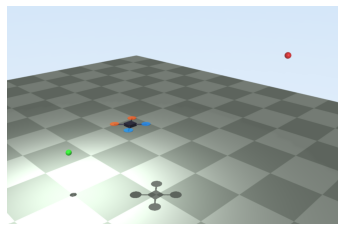
\includegraphics[width=0.46\linewidth]{mujoco_pointing_cell1.png}\hfill
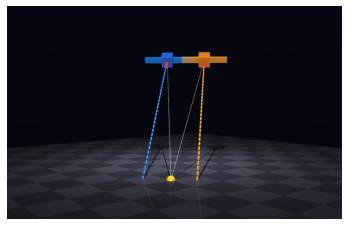
\includegraphics[width=0.46\linewidth]{mujoco_pointing_cell9.png}
\caption{MuJoCo scenes from the notebook: a quadrotor-shaped body flying to a goal (left) and the two bodies pointing their
lines of sight at a target (right).}
\label{fig:mujocoviews}
\end{figure}

\begin{toybox}[printed output of the Part-2 demo, $\|\qv\|$ every second]
\small
\begin{tabular}{@{}lcccccccccc@{}}
$t$ (s) & 0 & 1 & 2 & 3 & 4 & 5 & 6 & 7 & 8 & 9\\
constrained & 0.469 & 0.401 & 0.240 & 0.128 & 0.067 & 0.036 & 0.017 & 0.009 & 0.005 & 0.002\\
conventional PD & 0.469 & 0.401 & 0.214 & 0.031 & 0.048 & 0.040 & 0.016 & 0.003 & 0.007 & 0.006
\end{tabular}

The constrained body decays monotonically (no overshoot through zero); the PD body is sometimes ahead and then swings past
zero and back ($0.031\to0.048$). $\|\qv\|$ alone does not show the envelope, which is why the reproduction reports
$|\varepsilon|$ and the time outside (\cref{sec:part2}).
\end{toybox}

\subsection{MuJoCo: flight with altitude and attitude loops}

\code{Drones\_Mujoco\_Flying.ipynb} and \code{Drones\_Mujoco\_Good\_Trial.ipynb} add an altitude/position loop around the
attitude law on a quadrotor-shaped body with direct force and torque actuators (not four-rotor mixing).

\resfig{mujoco_flying_cell5.png}{0.6\linewidth}{MuJoCo flight: climb to 2\,m while the attitude quaternion converges from the
paper's Part-1 initial attitude.}{fig:mujocoflight}

The point-to-point flight from $(0,0,1)$ to $(3,3,3)$ (minimum-jerk reference over 6\,s, then 3\,s hover) prints its
position every 0.5\,s and ends at $(3.01,\ 3.01,\ 3.00)$\,m (\code{Drones\_Mujoco\_Good\_Trial.ipynb}). The flying notebook also
keeps our earlier unsuccessful attempts (wrong sign conventions in the position loop, cells 6--8) as development history;
they are not used as results.

\subsection{Interactive browser simulator}

\code{index.html} (with \code{app.js}, \code{simulation.js}) runs the rigid-body equations with RK4 in the browser and plots
quaternion, rate, torque and $\that$ live for the constrained law and PD. It uses the symmetric barrier form and is meant
for illustration in a presentation; it is not used for any number in this report.

% =====================================================================
\section{The MATLAB Toy Model}
\label{sec:toyguide}
% =====================================================================

The toy model is a set of small MATLAB scripts that make every block of the controller tangible: each one prints its
inputs and outputs with their sizes, units and meaning, reproduces the hand-calculated toy examples of the Mathematical
Models to six digits, and draws one figure that shows the idea. No toolbox is needed.

\subsection{The files}

\begin{center}\small
\begin{tabularx}{\linewidth}{@{}l l X@{}}
\toprule
\textbf{File in \code{toy\_model/}} & \textbf{Blocks} & \textbf{What you see when you run it}\\
\midrule
\code{step1\_ftppf.m} & 3 & $\rho_q(2)$ by hand; $\rho(0)=\rho_0$, $\rho(T_s)=\rho_T$, monotonicity; FTPPF vs.\ exponential PPF; effect of $T_s$ and $\kappa$\\
\code{step2\_normalised\_error.m} & 4, 5 & $\veps_1$, $\veps_2$ of the Part-1 state; barrier gains of both forms; the one-sided property\\
\code{step3\_control\_law.m} & 5, 2 & $\vs$, $\vu_{PD}$, $\vu_{cons}$, $\vu$, $\sat(\vu)$ at $t=0$; the three controllers on the same state\\
\code{step4\_adaptive\_law.m} & 6 & first Euler step by hand; $\that$ for a decaying and a persistent $\|\vs\|$; drift and the leakage floor\\
\code{step5\_single\_axis.m} & 1--6 & the whole idea on one axis ($J\ddot x=\sat(u)+d$): constrained vs.\ PD with the same gains and limit\\
\code{step6\_spacecraft\_closed\_loop.m} & 1--6 & independent re-implementation of the paper's Part 1 and Part 2 (cross-check of the Python numbers)\\
\code{step7\_x3\_mixer.m} & 10 & X3 allocation matrix from the SDF, hover speeds, torque authority, the v1 mixer error\\
\code{step8\_sampled\_data\_limit.m} & 9 & why the barrier gain must be capped on a 60\,Hz loop with one sample of delay\\
\code{run\_all.m} & all & runs steps 1--8, saves \code{figures/*.png} and the complete printed output in \code{results\_log.txt}\\
\code{lib/} & -- & \code{ftppf.m}, \code{control\_law.m}, \code{paper\_params.m}, \code{io\_print.m}, \code{step\_header.m}\\
\bottomrule
\end{tabularx}
\end{center}

\subsection{How to run them}

\begin{enumerate}[leftmargin=*]
  \item Open MATLAB and run \code{run('<repo>/toy\_model/run\_all.m')}, or open one step and press \emph{Run}. Every step adds
        \code{lib/} to the path itself, so it can be run on its own from any folder.
  \item Each step starts with a banner: step number, title and the equations of the block. Every printed line is tagged
        \code{[IN ]}, \code{[OUT]} or \code{[CHK]} and shows name, size, unit and meaning, followed by the value.
  \item The figures are written to \code{toy\_model/figures/}; this document includes them directly from there.
\end{enumerate}

\subsection{What the steps show}

\toyfig{step1_ftppf.png}{\linewidth}{Step 1: the finite-time property and the effect of $T_s$ and $\kappa$.}{fig:toy1}
\toyfig{step2_barrier_gain.png}{\linewidth}{Step 2: barrier gain of the paper form and the symmetric form, and the extra restoring
torque for $s=0.05$.}{fig:toy2}
\toyfig{step4_adaptive_law.png}{\linewidth}{Step 4: $\that$ for a decaying $\|\vs\|$, for a small persistent residual (drift),
and with a leakage floor $\eta_2\ge0.2$.}{fig:toy4}
\toyfig{step5_single_axis.png}{\linewidth}{Step 5: one axis, $J=1$, $|u|\le3$, $d=0.3\sin2t$. Same gains for both controllers;
only the constrained one stays inside the tube.}{fig:toy5}
\toyfig{step6_part2_constrained_vs_pd.png}{\linewidth}{Step 6: MATLAB re-implementation of the paper's Part 2.}{fig:toy6}
\toyfig{step6_part2_eps2.png}{0.8\linewidth}{Step 6: $\max_i|\varepsilon_{2i}|$ for the three controllers (MATLAB).}{fig:toy6b}
\toyfig{step7_x3_mixer.png}{\linewidth}{Step 7: torque produced per unit commanded by the v1 mixer and by the corrected mixer.}{fig:toy7}
\toyfig{step8_sampled_data_limit.png}{0.75\linewidth}{Step 8: spectral radius of the sampled roll, pitch and yaw loops against the
total gain on the rate.}{fig:toy8}

\subsection{Printed output}

\IfFileExists{../../toy_model/results_log.txt}{%
The complete output of \code{run\_all.m}, exactly as MATLAB printed it:
\lstinputlisting[style=common, basicstyle=\ttfamily\scriptsize, breaklines=true]{../../toy_model/results_log.txt}}{%
\code{run\_all.m} writes the complete printed output to \code{toy\_model/results\_log.txt}.}

\subsection{Things to try}

\begin{itemize}[leftmargin=*]
  \item In \code{step5}, set \code{S.alpha = 0; S.beta = 0;} to remove the barrier and compare the time outside the tube
        with the constrained run.
  \item In \code{step6}, set \code{P2.rq(1) = 0.3} (the paper's own Part-2 value): $\varepsilon_{11}(0)=1$ and the barrier gain is
        only finite because of the 0.999 guard ($1.5/0.001^2=1.5\times10^6$), finding P2.
  \item In \code{step6}, lower \code{P.umax} and watch when the envelope stops being feasible (\cref{sec:sens}).
  \item In \code{step8}, change \code{T = 1/60} to \code{1/250} and see how the stable range of the total gain grows.
\end{itemize}

% =====================================================================
\section{Conclusions and Scope of the Claims}
\label{sec:claims}
% =====================================================================

\subsection{What we have shown}

\begin{center}\small
\begin{longtable}{@{}p{7.3cm} p{6.9cm}@{}}
\toprule
\textbf{Claim} & \textbf{Evidence}\\
\midrule\endhead
Every equation of the paper (1)--(14), (22) is implemented and traceable to code. & Mathematical Models Section 6; \cref{sec:controller}.\\
The paper's Part~1 is reproduced: both states inside their envelopes for $T_s=15$ and 10\,s, faster convergence with the smaller $T_s$, torque within the limit. & \cref{tab:part1}, \cref{fig:part1}.\\
The paper's Part~2 is reproduced: at the same 2.5\,N\,m limit the constrained law stays inside both envelopes, conventional PD leaves the rate envelope 27.5\,\% of the time; the constrained law settles earlier with half the residual error and 36\,\% less torque energy. & \cref{tab:part2}, \cref{fig:part2w,fig:part2eps}.\\
The result is general within the paper's regime: 97.0\,\% violation-free over 300 random starts (PD: 0\,\%). & \cref{tab:mc}, study A.\\
Every toy example and every block can be re-run step by step in MATLAB, including an independent re-implementation of the spacecraft experiments. & \cref{sec:toyguide}, \cref{tab:crosscheck}.\\
The paper's barrier is one-sided; above the paper's disturbance level this costs constraint satisfaction, and a symmetric barrier removes the problem (97\,\% up to $3\times$ the disturbance). & \cref{sec:barrierform}, study B, X3 experiment E3.\\
The envelope must be feasible for the actuator; otherwise no controller can keep it. & \cref{tab:sens}, study C, E3b.\\
Our first Gazebo node crashed because of a mixer that did not match the X3 and an altitude-rate bug; both are identified by controlled experiments and fixed. & \cref{tab:e1}, \cref{tab:mixer}.\\
The paper's law, re-sized for the X3 and with a sampled-data gain cap, hovers for 180\,s and flies a 2\,m square (4\,cm RMS) with 0\,\% attitude-envelope violations on a software-in-the-loop X3 built from Gazebo's model files; under disturbance it cuts rate-envelope violations from 36\,\% (PD) to 6\,\% (paper form) or 0\,\% (symmetric form). & \cref{tab:e2,tab:e3,tab:e4}.\\
The ROS~2 node runs exactly this controller and passes the offline test against the surrogate. & \cref{sec:x3}, \code{tests/}.\\
\bottomrule
\end{longtable}
\end{center}

\subsection{What we do not claim}

\begin{itemize}[leftmargin=*]
  \item \textbf{A proof that the envelope is never left.} The paper's Theorem~1 proves convergence; constraint satisfaction is
        measured, and it does fail where the envelope is infeasible or the disturbance exceeds what the one-sided barrier
        handles.
  \item \textbf{Number-for-number agreement with the paper's figures.} The paper publishes plots only and leaves four values
        unstated; we match its behaviour and report our own numbers with the choices disclosed.
  \item \textbf{Results from a Gazebo log of the v2 node.} The X3 numbers in this document come from the software-in-the-loop
        surrogate (Gazebo's constants, 60\,Hz, one sample of delay, no sensor noise). Running \code{gazebo.py} in Gazebo
        and processing the log with \code{plot\_gazebo\_log.py} produces the same figures and metrics from the simulator itself
        (\cref{sec:setup}).
  \item \textbf{Hardware flight.} No physical vehicle was flown.
\end{itemize}

\subsection{Conclusion}

The constrained PD-type controller of Golestani et al.\ does what the paper says in the setting the paper uses: with the
same gains and the same saturated actuator as a conventional PD, it keeps both the attitude and the angular velocity inside
finite-time prescribed envelopes, converges faster and with less control effort, and it does so in 97\,\% of random
initial conditions, not only in the two cases shown in the paper. Its structure is as simple as claimed: our whole
implementation of the law is about twenty lines. Carrying it onto a quadcopter required three additions the paper does
not need (body rates from poses, an outer position loop, a correct motor mixer) and one change it does not anticipate (a cap
on the barrier gain for a 60\,Hz digital loop); with them the law flies the X3 model in hover and along a trajectory.
Two lessons go beyond the paper: the envelope must be chosen to be feasible for the actuator, and a two-sided barrier
is markedly more robust than the one-sided form printed in the paper.

\subsection{Future work}
\begin{enumerate}[leftmargin=*]
  \item Gazebo campaign with \code{gazebo.py}: hover, square and disturbance runs for the three controllers, compared with the
        surrogate numbers of \cref{sec:x3res}.
  \item An envelope-feasibility rule: choose $\rho_0,\rho_T,T_s$ from $\umax/\lambda_{\max}(J)$ and the expected disturbance.
  \item Rate-envelope scheduling for trajectory flight (widen $\rho_\omega$ during manoeuvres).
  \item Actuator rate limits, which the paper itself names as future work.
\end{enumerate}

\appendix
% =====================================================================
\section{Appendix}
\label{sec:appendix}
% =====================================================================

\subsection{Where every figure and number comes from}

\begin{center}\small
\begin{longtable}{@{}p{5.4cm} p{5.6cm} p{3.0cm}@{}}
\toprule
\textbf{Output} & \textbf{Written by} & \textbf{Used in}\\
\midrule\endhead
\code{fig01\_ppf\_comparison.png} & \code{paper\_reproduction.py} & \cref{fig:ppf}\\
\code{fig02\_part1\_Ts15/Ts10.png}, \code{fig03} & \code{paper\_reproduction.py} & \cref{sec:part1}\\
\code{fig04}--\code{fig08} & \code{paper\_reproduction.py} & \cref{sec:part2}\\
\code{fig09\_barrier\_forms.png} & \code{paper\_reproduction.py} & \cref{sec:barrierform}\\
\code{fig10}, \code{fig11} & \code{paper\_reproduction.py} & \cref{sec:beyond}\\
\code{results/metrics.md}, \code{.json} & \code{paper\_reproduction.py} & \cref{sec:repro,sec:beyond}\\
\code{x3\_E0}--\code{x3\_E4} figures & \code{x3\_sim/run\_x3\_experiments.py} & \cref{sec:x3res}\\
\code{results/x3\_metrics.md}, \code{.json} & \code{x3\_sim/run\_x3\_experiments.py} & \cref{sec:x3,sec:x3res}\\
\code{toy\_model/figures/*.png}, \code{results\_log.txt} & \code{toy\_model/run\_all.m} (MATLAB) & \cref{sec:toyguide,sec:crosscheck}\\
\code{mujoco\_*.png} & MuJoCo notebooks (outputs exported) & \cref{sec:demos}\\
\code{flow\_paper.pdf}, \code{flow\_x3.pdf} & \code{mathematical\_models/figures/*.tex} & \cref{fig:flowpaper,fig:flowx3}\\
\code{gazebo\_<mode>\_<exp>.png/.json} & \code{plot\_gazebo\_log.py} from a Gazebo run & --\\
\bottomrule
\end{longtable}
\end{center}

\subsection{All parameters in one place}

\begin{center}\small
\begin{tabularx}{\linewidth}{@{}l X@{}}
\toprule
\textbf{Group} & \textbf{Values}\\
\midrule
Spacecraft (paper) & $J=[20,1.2,0.9;\,1.2,17,1.4;\,0.9,1.4,15]$\,kg\,m$^2$; $\umax=2.5$\,N\,m; $\vd(t)=[0.05\sin t,\,0.1\sin1.2t,\,0.15\sin1.5t]$\,N\,m\\
Law (paper) & $k_p=40$, $k_d=20$, $\alpha=1.5$, $\beta=1.2$, $\eta_1=0.1$, $\eta_2=2e^{-0.5t}$, $\that(0)=0$\\
Envelope (paper) & $\rho_q:0.3\to0.008$, $\rho_\omega:0.4\to0.005$\,rad/s, $\kappa=2.5$, $T_s=15$ or $10$\,s\\
Unstated (ours) & $c=0.5$, $\varsigma=0.02$, Part 2: $T_s=15$\,s, $\rho_{q0}=0.36$\\
Simulation & RK4, 1\,ms, ZOH torque, 20\,s; Monte-Carlo $N=300$, seed 7\\
X3 vehicle & $m=1.52$\,kg, $J=\diag(0.03565,0.07035,0.09892)$\,kg\,m$^2$, $k_T=8.54858\times10^{-6}$, $c_Q=0.016$, $\Omega_{\max}=800$\,rad/s\\
X3 law & $k_p=4$, $k_d=0.4$, $\alpha=0.15$, $\beta=0.12$, $c=1$, $\varsigma=0.5$, $\eta_1=5$, $\eta_2\ge0.2$, $\that\le0.1$, $g_{\max}=1$, $|\tau|\le0.35$\,N\,m\\
X3 envelope & $\rho_q:0.30\to0.02$, $\rho_\omega:2.5\to0.05$\,rad/s, $\kappa=2$, $T_s=10$\,s\\
X3 outer loop & $K_{p,z}=5$, $K_{d,z}=3.5$, $K_{p,xy}=1.2$, $K_{d,xy}=1.6$, tilt $\le0.35$\,rad; rate filter 0.6, velocity filter 0.3\\
\bottomrule
\end{tabularx}
\end{center}

\subsection{References}
\begin{enumerate}[leftmargin=*]
  \item M.~Golestani, K.~A.~Alattas, S.~Ud~Din, S.~Mobayen, A.~K.~Alanazi, A.~Fekih, ``A Simple Structure Constrained Attitude
        Control for Rigid Bodies: A PD-Type Control,'' \emph{IEEE Access}, vol.~10, pp.~10202--10209, 2022,
        doi:10.1109/ACCESS.2022.3144627.
  \item C.~P.~Bechlioulis, G.~A.~Rovithakis, ``Robust adaptive control of feedback linearizable MIMO nonlinear systems with
        prescribed performance,'' \emph{IEEE Trans.\ Autom.\ Control}, vol.~53, no.~9, pp.~2090--2099, 2008.
  \item J.~T.-Y.~Wen, K.~Kreutz-Delgado, ``The attitude control problem,'' \emph{IEEE Trans.\ Autom.\ Control}, vol.~36, no.~10,
        pp.~1148--1162, 1991.
  \item H.~K.~Khalil, \emph{Nonlinear Systems}, 3rd ed., Prentice Hall, 2002.
  \item Z.~Chen, J.~Huang, ``Attitude tracking and disturbance rejection of rigid spacecraft by adaptive control,''
        \emph{IEEE Trans.\ Autom.\ Control}, vol.~54, no.~3, pp.~600--605, 2009. (Source of the paper's inertia matrix.)
  \item Gazebo Sim: \code{quadcopter.sdf} example world and the \code{MulticopterMotorModel} system.
  \item E.~Todorov, T.~Erez, Y.~Tassa, ``MuJoCo: A physics engine for model-based control,'' IROS 2012.
\end{enumerate}


\end{document}
